\documentclass[12pt,a4paper,twoside,openright]{report}
\let\openright=\cleardoublepage

%%% Choose a language %%%

\newif\ifEN
\ENtrue   % uncomment this for english
%\ENfalse   % uncomment this for czech

%%% Configuration of the title page %%%

% \def\ThesisTitleStyle{mff} % MFF style
%\def\ThesisTitleStyle{cuni} % uncomment for old-style with cuni.cz logo
\def\ThesisTitleStyle{natur} % uncomment for nature faculty logo

% \def\UKFaculty{Faculty of Mathematics and Physics}
\def\UKFaculty{Faculty of Science}

\def\UKName{Charles University in Prague} % this is not used in the "mff" style

% Thesis type names, as used in several places in the title
\def\ThesisTypeTitle{\ifEN BACHELOR THESIS \else BAKALÁŘSKÁ PRÁCE \fi}
%\def\ThesisTypeTitle{\ifEN MASTER THESIS \else DIPLOMOVÁ PRÁCE \fi}
%\def\ThesisTypeTitle{\ifEN RIGOROUS THESIS \else RIGORÓZNÍ PRÁCE \fi}
%\def\ThesisTypeTitle{\ifEN DOCTORAL THESIS \else DISERTAČNÍ PRÁCE \fi}
\def\ThesisGenitive{\ifEN bachelor \else bakalářské \fi}
%\def\ThesisGenitive{\ifEN master \else diplomové \fi}
%\def\ThesisGenitive{\ifEN rigorous \else rigorózní \fi}
%\def\ThesisGenitive{\ifEN doctoral \else disertační \fi}
\def\ThesisAccusative{\ifEN bachelor \else bakalářskou \fi}
%\def\ThesisAccusative{\ifEN master \else diplomovou \fi}
%\def\ThesisAccusative{\ifEN rigorous \else rigorózní \fi}
%\def\ThesisAccusative{\ifEN doctoral \else disertační \fi}



%%% Fill in your details %%%

% (Note: \xxx is a "ToDo label" which makes the unfilled visible. Remove it.)
\def\ThesisTitle{Differential discovery of protein features using tandem mass spectrometer}
\def\ThesisAuthor{Evžen Wybitul}
\def\YearSubmitted{2021}

% department assigned to the thesis
\def\Department{Department of Cell Biology}
% Is it a department (katedra), or an institute (ústav)?
\def\DeptType{Department}

\def\Supervisor{Miroslav Kratochvíl}
\def\SupervisorsDepartment{\xxx{Noxemchâteau Apartment}}

% Study programme and specialization
\def\StudyProgramme{Bioinformatics}
\def\StudyBranch{Bioinformatics}

\def\Dedication{%
  Dedication. First and foremost, I thank my supervisor and former colleague RNDr. Miroslav Kratochvíl, Ph.D., for his guidance and assistance during my research and during the writing of this thesis.

  I thank doc. RNDr. Josef Cvačka, Ph.D., for providing the testing data. Mgr. Martin Hubálek, Ph.D., has my sincerest thanks for relentlessly answering my many questions related to mass spectrometry.

  My dear Lucka deserves special gratitude for enduring the many unsolicited mini-lectures about fragmentation in mass spectrometry, and for always being there for me when I needed it.

  Last but not least, I am grateful to my parents for their perpetual support throughout my studies at the university, and for the many compromises they had to make in order for me to successfully finish writing this thesis.
}

\def\AbstractEN{%
  Disulphide bonds are crucial to correct protein folding, and heavily influence protein function. Tandem mass spectrometry protein analysis is often used for the determination of disulphide bond positions, in combination with manual or computational interpretation methods. In this thesis we devise a program for automatic disulphide bond characterization called Dibby. Dibby identifies protein fragments in the fragmentation spectra, and uses the identified fragments to determine which cysteines were connected in the protein. The identification algorithm is able to identify even complex fragments with multiple disulphide bonds that are often missed by other methods. To reduce the fragment search space, we employ divide and conquer and branch and bound techniques. We evaluate Dibby on both measured and in-silico generated datasets, and find that it correctly identifies large portion of the present disulphide bonds with minimal manual interventions.
}

\def\AbstractCS{%
  Disulfidické můstky hrají důležitou roli při skládání proteinů a mají velký vliv na jejich funkci. K určování polohy disulfidických můstků v proteinech se často používá tandemová hmotnostní spektrometrie v kombinaci s manuální nebo výpočetní interpretací výsledků. V této práci představujeme progam Dibby, který má za cíl charakterizovat disulfidické můstky v proteinu. Dibby identifikuje proteinové fragmenty ve fragmentačních spektrech a s jejich pomocí určuje, kde v proteinu se disulfidické můstky nacházejí. Použitý identifikační algoritmus zvládá identifikovat i komplexní fragmenty s několika disulfidickými můstky, kterých si jiné metody často nevšimnou. Abychom při identifikaci fragmentů zmenšili vyhledávací prostor, využíváme metodu rozděl a panuj a metodu větví a mezí. Pomocí evaluace na naměřených i na uměle vygenerovaných datasetech jsme ověřili, že Dibby jen s minimálními manuálními zásahy správně rozpozná velkou část přítomných disulfidických můstků.
}

% 3 to 5 keywords (recommended), each enclosed in curly braces.
% Keywords are useful for indexing and searching for the theses by topic.
\def\Keywords{%
  {mass spectrometry}, {disulphide bonds}, {disulphide bond mapping}, {fragmentation spectra labelling}
}

% If your abstracts are long and do not fit in the infopage, you can make the
% fonts a bit smaller by this setting. (Also, you should try to compress your abstract more.)
% Alternatively, consider increasing the size of the page by uncommenting the
% geometry modification in thesis.tex.
\def\InfoPageFont{}
%\def\InfoPageFont{\small}  %uncomment to decrease font size

\usepackage[a-2u]{pdfx}

\ifEN\else\usepackage[czech,shorthands=off]{babel}\fi
\usepackage[utf8]{inputenc}
\usepackage[T1]{fontenc}

% See https://en.wikipedia.org/wiki/Canons_of_page_construction before
% modifying the size of printable area. LaTeX defaults are great.
% If you feel it would help anything, you can enlarge the printable area a bit:
%\usepackage[textwidth=390pt,textheight=630pt]{geometry}
% The official recommendation expands the area quite a bit (looks pretty harsh):
%\usepackage[textwidth=145mm,textheight=247mm]{geometry}

%%% FONTS %%%
\usepackage{lmodern} % TeX "original" (this sets up the latin mono)

% Optionally choose an override for the main font for typesetting
\usepackage[mono=false]{libertinus} % popular for comp-sci (ACM uses this)
%\usepackage{tgschola} % Schoolbook-like (gives a bit of historic feel)
%\usepackage[scale=0.96]{tgpagella} % Palladio-like (popular in formal logic).

% Optionally choose a custom sans-serif fonts (e.g. for figures and tables).
% Default sans-serif font is usually Latin Modern Sans. Some font packages
% (e.g. libertinus) replace that with a better matching sans-serif font.
%\usepackage{tgheros} % recommended and very readable (Helvetica-like)
%\usepackage{FiraSans} % looks great
% DO NOT typeset the main text in sans-serif font!
% The serifs make the text easily readable on the paper.

% IMPORTANT FONT NOTE: Some fonts require additional PDF/A conversion using
% the pdfa.sh script. These currently include only 'tgpagella'; but various
% other fonts from the texlive distribution need that too (mainly the Droid
% font family).

% Packages added by me
\usepackage[version=4]{mhchem}
\usepackage{textcomp}
\usepackage{rotating}
\usepackage{multirow}
\usepackage{mathtools}
\usepackage{microtype}

\DeclarePairedDelimiterX\set[1]\lbrace\rbrace{\def\given{\;\delimsize\vert\;}#1}


% some useful packages
\usepackage{amsmath,amsfonts,amsthm,bm}
\usepackage{graphicx}
\usepackage{xcolor}
\usepackage{booktabs}
\usepackage{caption}
\usepackage{floatrow}

% load bibliography tools
\usepackage[backend=bibtex,natbib,style=numeric,sorting=none]{biblatex}
% alternative with alphanumeric citations (more informative than numbers):
%\usepackage[backend=bibtex,natbib,style=alphabetic]{biblatex}
%
% alternatives that conform to iso690
% (iso690 is not formally required on MFF, but may help elsewhere):
%\usepackage[backend=bibtex,natbib,style=iso-numeric,sorting=none]{biblatex}
%\usepackage[backend=bibtex,natbib,style=iso-alphabetic]{biblatex}
%
% additional option choices:
%  - add `giveninits=true` to typeset "E. A. Poe" instead of full Edgar Allan
%  - `terseinits=true` additionaly shortens it to nature-like "Poe EA"
%  - add `maxnames=10` to limit (or loosen) the maximum number of authors in
%    bibliography entry before shortening to `et al.` (useful when referring to
%    book collections that may have hundreds of authors)
%  - for additional flexibility (e.g. multiple reference sections, etc.),
%    remove `backend=bibtex` and compile with `biber` instead of `bibtex` (see
%    Makefile)
%  - `sorting=none` causes the bibliography list to be ordered by the order of
%    citation as they appear in the text, which is usually the desired behavior
%    with numeric citations. Additionally you can use a style like
%    `numeric-comp` that compresses the long lists of citations such as
%    [1,2,3,4,5,6,7,8] to simpler [1--8]. This is especially useful if you plan
%    to add tremendous amounts of citations, as usual in life sciences and
%    bioinformatics.
%  - if you don't like the "In:" appearing in the bibliography, use the
%    extended style (`ext-numeric` or `ext-alphabetic`), and add option
%    `articlein=false`.
%
% possibly reverse the names of the authors with the default styles:
%\DeclareNameAlias{default}{family-given}

% load the file with bibliography entries
\addbibresource{refs}

% remove this if you won't use fancy verbatim environments
\usepackage{fancyvrb}

% remove this if you won't typeset TikZ graphics
\usepackage{tikz}
\usetikzlibrary{positioning} %add libraries as needed (shapes, decorations, ...)

% remove this if you won't typeset any pseudocode
\usepackage{algpseudocode}[noend]
\usepackage{algorithm}[noend]

% remove this if you won't list any source code
\usepackage{listings}


\hypersetup{unicode}
\hypersetup{breaklinks=true}

\usepackage[noabbrev]{cleveref}

\input{todos} % remove this before compiling the final version


% use this for typesetting a chapter without a number, e.g. intro and outro
\def\chapwithtoc#1{
  \chapter*{#1}
  \addcontentsline{toc}{chapter}{#1}
}

% If there is a line/figure overflowing into page margin, this will make the
% problem evident by drawing a thick black line at the overflowing spot. You
% should not disable this.
\overfullrule=0mm

% The maximum stretching of a space. Increasing this makes the text a bit more
% sloppy, but may prevent the overflows by moving words to next line.
\emergencystretch=1em

\ifEN
  \theoremstyle{plain}
  \newtheorem{thm}{Theorem}
  \newtheorem{lemma}[thm]{Lemma}
  \newtheorem{claim}[thm]{Claim}
  \newtheorem{defn}{Definition}
  \theoremstyle{remark}
  \newtheorem*{cor}{Corollary}
\else
  \theoremstyle{plain}
  \newtheorem{thm}{Věta}
  \newtheorem{lemma}{Lemma}
  \newtheorem{claim}{Tvrzení}
  \newtheorem{defn}{Definice}
  \theoremstyle{remark}
  \newtheorem*{cor}{Důsledek}
\fi

\newenvironment{myproof}{
  \par\medskip\noindent
  \textit{\ifEN Proof \else Důkaz \fi}.
}{
  \newline
  \rightline{$\qedsymbol$}
}

% real/natural numbers
\newcommand{\R}{\mathbb{R}}
\newcommand{\N}{\mathbb{N}}

% asymptotic complexity
\newcommand{\asy}[1]{\mathcal{O}(#1)}

% listings and default lstlisting config (remove if unused)
\DeclareNewFloatType{listing}{}
\floatsetup[listing]{style=ruled}

\DeclareCaptionStyle{thesis}{style=base,font={small,sf},labelfont=bf,labelsep=quad}
\captionsetup{style=thesis}
\captionsetup[algorithm]{style=thesis,singlelinecheck=off}
\captionsetup[listing]{style=thesis,singlelinecheck=off}

% \setcounter{secnumdepth}{4}
\titleformat{\chapter}{\fontsize{24pt}{24pt}\bfseries}{\color{black!25}\thechapter.}{1em}{}
\titleformat{\section}{\fontsize{16pt}{18pt}\bfseries}{\color{black!25}\thesection}{1em}{}
\titleformat{\subsection}{\fontsize{14pt}{16pt}\bfseries}{\color{black!25}\thesubsection}{1em}{}
\titleformat{\subsubsection}{\bfseries}{\color{black!25}\thesubsubsection}{1em}{}

% Uncomment for table captions on top. This is sometimes recommended by the
% style guide, and even required for some publication types.
%\floatsetup[table]{capposition=top}
%
% (Opinionated rant:) Captions on top are not "compatible" with the general
% guideline that the tables should be formatted to be quickly visually
% comprehensible and *beautiful* in general (like figures), and that the table
% "head" row (with column names) should alone communicate most of the content
% and interpretation of the table. If you just need to show a long boring list
% of numbers (because you have to), either put some effort into showing the
% data in an attractive figure-table, or move the data to an attachment and
% refer to it, so that the boredom does not impact the main text flow.
%
% You can make the top-captions look much less ugly by aligning the widths of
% the caption and the table, with setting `framefit=yes`, as shown below.  This
% additionally requires some extra markup in your {table} environments; see the
% comments in the example table in `ch2.tex` for details.
%\floatsetup[table]{capposition=top,framefit=yes}

\ifEN\floatname{listing}{Listing}
\else\floatname{listing}{Výpis kódu}\fi
\lstset{ % use this to define styling for any other language
  language=C++,
  tabsize=2,
  showstringspaces=false,
  basicstyle=\footnotesize\tt\color{black!75},
  identifierstyle=\bfseries\color{black},
  commentstyle=\color{green!50!black},
  stringstyle=\color{red!50!black},
  keywordstyle=\color{blue!75!black}}

\newcommand{\nb}[1] {\State\triangleright\>#1}
\newcommand{\Decl}[2] {\State $\mathit{#1} \gets$ #2}
\newcommand{\Upd}[2] {\State $\mathit{#1} \mathrel{{+}{=}}$ #2}
\newcommand{\Var}[1] {$\mathit{#1}$}

% Czech versions of the used cleveref references (It's not as convenient as in
% English because of declension, cleveref is limited to sg/pl nominative. Use
% plain \ref to dodge that.)
\ifEN\relax\else
  \crefname{chapter}{kapitola}{kapitoly}
  \Crefname{chapter}{Kapitola}{Kapitoly}
  \crefname{section}{sekce}{sekce}
  \Crefname{section}{Sekce}{Sekce}
  \crefname{subsection}{sekce}{sekce}
  \Crefname{subsection}{Sekce}{Sekce}
  \crefname{subsubsection}{sekce}{sekce}
  \Crefname{subsubsection}{Sekce}{Sekce}
  \crefname{figure}{obrázek}{obrázky}
  \Crefname{figure}{Obrázek}{Obrázky}
  \crefname{table}{tabulka}{tabulky}
  \Crefname{table}{Tabulka}{Tabulky}
  \crefname{listing}{výpis}{výpisy}
  \Crefname{listing}{Výpis}{Výpisy}
  \floatname{algorithm}{Algoritmus}
  \crefname{algorithm}{algoritmus}{algoritmy}
  \Crefname{algorithm}{Algoritmus}{Algoritmy}
  \newcommand{\crefpairconjunction}{ a~}
  \newcommand{\crefrangeconjunction}{ a~}
\fi
 % use this file for various custom definitions


\begin{document}

% % the layout is mandatory, edit only in dire circumstances

\pagestyle{empty}
\hypersetup{pageanchor=false}
\begin{center}

  % top part of the layout, this actually differs between faculties

  \def\ThesisTitleXmff{%
    \ifEN
      \centerline{\mbox{\includegraphics[width=166mm]{img/logo-en.pdf}}}
    \else
      \centerline{\mbox{\includegraphics[width=166mm]{img/logo-cs.pdf}}}
    \fi
    \vspace{-8mm}\vfill%
    {\bf\Large\ThesisTypeTitle}
    \vfill%
    {\LARGE\ThesisAuthor}\par
    \vspace{15mm}%
    {\LARGE\bfseries\ThesisTitle}%
    \vfill%
    \Department}
  \def\ThesisTitleCuniLogo#1{%
    {\large\UKName\par\medskip\par\UKFaculty }
    \vfill%
    {\bf\Large\ThesisTypeTitle}
    \vfill%
    \includegraphics[width=70mm]{#1}
    \vfill%
    {\LARGE\ThesisAuthor}\par
    \vspace{15mm}%
    {\LARGE\bfseries\ThesisTitle}
    \vfill%
    \Department\par}
  \def\ThesisTitleXcuni{\ThesisTitleCuniLogo{img/uklogo.pdf}}
  \def\ThesisTitleXnatur{\ThesisTitleCuniLogo{img/naturlogo.pdf}}

  % choose the correct page and print it
  \csname ThesisTitleX\ThesisTitleStyle\endcsname
  % latex corner: X is the new @

  \vfill

  {
    \centerline{\vbox{\halign{\hbox to 0.45\hsize{\hfil #}&\hskip 0.5em\parbox[t]{0.45\hsize}{\raggedright #}\cr
          \ifEN Supervisor of the thesis:
          \else Vedoucí \ThesisGenitive práce: \fi
          & \Supervisor \cr
          \noalign{\vspace{2mm}}
          \ifEN Study programme: \else Studijní program: \fi
          & \StudyProgramme \cr
          \noalign{\vspace{2mm}}
          \ifEN Study branch: \else Studijní obor: \fi
          & \StudyBranch \cr
        }}}}

  \vfill

  \ifEN Prague \else Praha \fi
  \YearSubmitted

\end{center}

\newpage

% remember to sign this!
\openright
\hypersetup{pageanchor=true}
\pagestyle{plain}
\pagenumbering{roman}
\vglue 0pt plus 1fill

\ifEN
  \noindent
  I declare that I carried out this \ThesisAccusative thesis independently, and only with the cited
  sources, literature and other professional sources. It has not been used to obtain another
  or the same degree.
\else
  \noindent
  Prohlašuji, že jsem tuto \ThesisAccusative práci vypracoval(a) samostatně a výhradně
  s~použitím citovaných pramenů, literatury a dalších odborných zdrojů.
  Tato práce nebyla využita k získání jiného nebo stejného titulu.
\fi

\ifEN
  \medskip\noindent
  I understand that my work relates to the rights and obligations under the Act No.~121/2000 Sb.,
  the Copyright Act, as amended, in particular the fact that the Charles
  University has the right to conclude a license agreement on the use of this
  work as a school work pursuant to Section 60 subsection 1 of the Copyright~Act.
\else
  \medskip\noindent
  Beru na~vědomí, že se na moji práci vztahují práva a povinnosti vyplývající
  ze zákona č. 121/2000 Sb., autorského zákona v~platném znění, zejména skutečnost,
  že Univerzita Karlova má právo na~uzavření licenční smlouvy o~užití této
  práce jako školního díla podle §60 odst. 1 autorského zákona.
\fi

\vspace{10mm}


\ifEN
  \hbox{\hbox to 0.5\hsize{%
      In \hbox to 6em{\dotfill} date \hbox to 6em{\dotfill}
      \hss}\hbox to 0.5\hsize{\dotfill\quad}}
  \smallskip
  \hbox{\hbox to 0.5\hsize{}\hbox to 0.5\hsize{\hfil Author's signature\hfil}}
\else
  \hbox{\hbox to 0.5\hsize{%
      V \hbox to 6em{\dotfill} dne \hbox to 6em{\dotfill}
      \hss}\hbox to 0.5\hsize{\dotfill\quad}}
  \smallskip
  \hbox{\hbox to 0.5\hsize{}\hbox to 0.5\hsize{\hfil Podpis autora\hfil}}
\fi

\vspace{20mm}
\newpage

% dedication

\openright

\noindent
\Dedication

\newpage

% mandatory information page

\openright

\vbox to 0.49\vsize{\InfoPageFont
  \setlength\parindent{0mm}
  \setlength\parskip{5mm}

  \ifEN Title: \else Název práce: \fi
  \ThesisTitle

  \ifEN Author: \else Autor: \fi
  \ThesisAuthor

  \DeptType:
  \Department

  \ifEN Supervisor: \else Vedoucí bakalářské práce: \fi
  \Supervisor, \SupervisorsDepartment

  \ifEN Abstract: \AbstractEN \else Abstrakt: \AbstractCS \fi

  \ifEN Keywords: \else Klíčová slova: \fi
  \Keywords

  \vss}\ifEN\relax\else\nobreak\vbox to 0.49\vsize{\InfoPageFont
    \setlength\parindent{0mm}
    \setlength\parskip{5mm}

    Title:
    \ThesisTitleEN

    Author:
    \ThesisAuthor

    \DeptTypeEN:
    \DepartmentEN

    Supervisor:
    \Supervisor, \SupervisorsDepartmentEN

    Abstract:
    \AbstractEN

    Keywords:
    \KeywordsEN

    \vss}
\fi

\newpage

\openright
\pagestyle{plain}
\pagenumbering{arabic}
\setcounter{page}{1}


\tableofcontents


\chapwithtoc{Introduction}

\begin{enumerate}
  \item Existují proteiny, jsou klíčové pro funkci organismu, obstarávají většinu procesů v něm. Funkce proteinu je závislá na jejich struktuře, a ta je závislá mimo jiné i na nekovalentních interakcích jednotlivých aminokyselin. Tyto interakce probíhají přes vodíkové nebo disulfidické můstky.
  \item Vědět, kde tyto můstky jsou, může pomoci molecular dynamic simulations pro omezení vyhledávacího prostoru, propř. určitě i jiným věcem.
  \item Metod určování pozic SS můstků existuje spousta. Jedna z nich využívá tandemovou hmotnostní spektrometrii v kombinaci s kapalinovou chromatografií. To vše na částečně alkylovaném proteinu, který je rozložený trypsinem.
  \item V této práci jsme zvolili podobný postup (to jest LC-MSMS na tryptických peptidech), ale přidali jsme k němu in-silico matchování (di)peptidů na naměřená spektra pomocí novel divide and conquer metody. Tato metoda využívá toho, že dipeptidy mají specifický fragmentační pattern a navíc mají i jinou prekurzorovou hmotu.
  \item Tuto metodu ověřujeme na několika naměřených proteinech, a máme svkělé výsledky (hopefully).
\end{enumerate}


% Introduction should answer the following questions, ideally in this order:
% \begin{enumerate}
% \item What is the nature of the problem the thesis is addressing?
% \item What is the common approach for solving that problem now?
% \item How this thesis approaches the problem?
% \item What are the results? Did something improve?
% \item What can the reader expect in the individual chapters of the thesis?
% \end{enumerate}

% Expected length of the introduction is between 1--4 pages. Longer introductions may require sub-sectioning with appropriate headings --- use \texttt{\textbackslash{}section*} to avoid numbering (with section names like `Motivation' and `Related work'), but try to avoid lengthy discussion of anything specific. Any ``real science'' (definitions, theorems, methods, data) should go into other chapters.
% \todo{You may notice that this paragraph briefly shows different ``types'' of `quotes' in TeX, and the usage difference between a hyphen (-), en-dash (--) and em-dash (---).}

% It is very advisable to skim through a book about scientific English writing before starting the thesis. I can recommend `\citetitle{glasman2010science}' by \citet{glasman2010science}.

\chapter{Tandem mass spectrometry in the context of disulfide bond analysis}

In the introduction we have established that disulfide bonds (DB) are important to protein function, structure, and to enzyme regulation. We have also shown that information about their positions can be used to optimise folding methods that are based on molecular dynamic simulations. We hope that these are enough to persuade the reader that studying the DB positions in a protein is a worthwhile task, although a complicated one.

There are many methods aiming to determine the positions of DBs; the most popular is tandem mass spectrometry (MS/MS). MS/MS is a popular analysis technique, often used in proteomics, and specifically DB mapping, for its accuracy, sensitivity and speed.~\cite{gorman2002protein}

In MS/MS analysis (or more accurately its bottom-up variant), the protein is eventually fragmented to smaller charged peptides whose mass to charge ratio (\(m/z\)) is measured with atomic precision. Multiple sets of \emph{fragmentation spectra} are obtained, each coming from a longer peptide with a specific \(m/z\) value that is called the \emph{precursor}. While in proteomics the task is usually to identify the original protein from the fragments, during DB mapping it is known which protein the fragments come from, and instead the task is to determine the positions of its DBs.

The experiment can be designed in a way that keeps the DBs intact, resulting in the occurence of crosslinked peptides with specific fragmentation signatures. There are multiple analytical methods, both manual and computational, that try to discover these fragmentation spectra and use them to determine the positions of the DBs in the protein. Other methods choose to dissociate the DBs during the fragmentation, a process that leads to another kind of specific fragmentation signatures.

The first few sections of this chapter roughly reflect the first few steps in a mass spectrometry experiment.

\begin{enumerate}
  \item The first topic we discuss is sample preparation, an important prerequisite in bottom-up mass spectrometric analysis (\Cref{sec:trypsin}).
  \item In \Cref{sec:lc}, a short overview of sample separation methods is provided.
  \item With the sample being digested and separated, we move on to explain the principles behind mass spectrometry itself, putting the focus on methods and techniques that are relevant to disulfide bond analysis (\Cref{sec:msms}). Where possible, we compare multiple methods and state their tradeoffs in the context of our work.
  \item Finally, we list some of the current approaches to DB mapping, noting their respective strengths and weaknesses (\Cref{sec:analysis}). At the very end of this chapter, we reformulate the task in more formal terms and roughly approximate its computational complexity.
\end{enumerate}

\section{Protein digestion and sample preparation}\label{sec:trypsin}

In order for the protein to be analysed, it first needs to be digested into smaller peptides; trypsin, and, to a lesser extent, pepsin, are popular choices in general proteomics.

Trypsin is a serine protease that cleaves amino acid chains at the carboxyllic side of lysine and arginine, provided they are not followed by proline~\cite{olsen2004trypsin}. Lysine and arginine are both relatively abundant in most proteins which makes the tryptic digestion peptides --- or as we will call them, \emph{tryptides} --- reasonably sized for a mass spectrometry analysis~\cite{matthiesen2020trypticsize}. Additionally, trypsin has very high specificity, and thus the digestion peptides are quite predictable. That being said, the sample protein is not cleaved at every potential cleavage site; so called \emph{missed cleavages} do occur during most proteolytic digestions. The frequency of missed cleavages depends on neigbouring residues of the cleavage site~\cite{gershon2014cleaved}, the used protease, and the experimental setup.

Relevant to our work is the following particularity of trypsin and some other proteases: they require a neutral-to-basic environment in order to become proteolytically active. In this environment the issue of DB scrambling arises~\cite{wu1997novel}; some of the DBs become dissociated, then the cysteines re-connect, but in different patterns than before. These scrambled bonds are diffucult to discern from the naturally occuring ones in the mass spectra. The issue can be mitigated by using a different protease for the digestion, such as pepsin, or thermolysin~\cite{sung2016evaluation}.

In addition to digestion, in a general proteomic experiment the protein usually undergoes reduction that completely dissociates the DBs, and cysteine alkylation that prevents the cysteines from reassociating. However, in an experiment that aims to characterise cysteine linkages, only the alkylation is performed, and the present DBs are kept intact.

\section{Liquid chromatography sample separation}\label{sec:lc}

In a general proteomic experiment, the signal from more abundant sample peptides may interfere with the other, less frequent ones. To sidestep this problem, it has become routine to perform separation before the main MS experiment, either on the protein level or the peptide level. After separation, less analytes are present in a mass spectrometer at a given point in time, reducing the chance of a signal becoming lost. Protein-level separation is common among experiments with the goal of identifying which proteins are present in the sample; in the case of disulfide bond characterisation, there is only one protein present, so peptide-level separation is the method of choice.

A popular peptide-level separation method is liquid chromatography (LC). In a model proteomic MS-LC experiment, the proteins are digested without prior separation, and the resulting peptides are separated on reverse-phase liquid chromatography column that is directly connected to a tandem mass spectrometer~\cite{washburn2001large}. This process is applicable to DB analysis as well.

Reverse-phase LC has two main constituents: a mobile liquid phase that contains the peptides, and a stationary solid phase which is usually a nonpolar column with \(\ce{C18}\) alkyl chains~\cite{chang1976high}. The mobile phase passes along the stationary phase, the elution time of each individual peptide depending on its hydrophobic interactions with the alkyls. The peptides are eluted with a polar mixture of water and organic solvent, such as acetonitrile~\cite{frohlich2006proteome}, the shortest and least hydrophilic peptides eluting the earliest.

The LC column is often directly connected to the mass spectrometer, which performs the bulk of the analysis.


\section{Tandem mass spectrometry}\label{sec:msms}

Mass spectrometry is an analytical technique that has originally been used for studying small thermostable molecules. Nevertheless, with the advancements in soft ionization allowing proteins and other biomolecules to be analysed as well~\cite{fenn1989electrospray}, mass spectrometry has become an indispesable tool in proteomics research~\cite{collins2003human}.

Mass spectrometry experiments can be either single-stage (MS) or tandem, the latter being denominated MS/MS, sometimes MS\textsuperscript{2}, and in the cases of more than two subsequent analyses, MS\textsuperscript{\(n\)}. During single-stage experiments, the mass distribution of a polypeptide sample is determined. The more frequent of the two, tandem mass spectrometry is used to learn about certain structural features of a protein, including sequence and post-translational modifications.~\cite{domon2006mass}

\begin{figure}
  \centering
  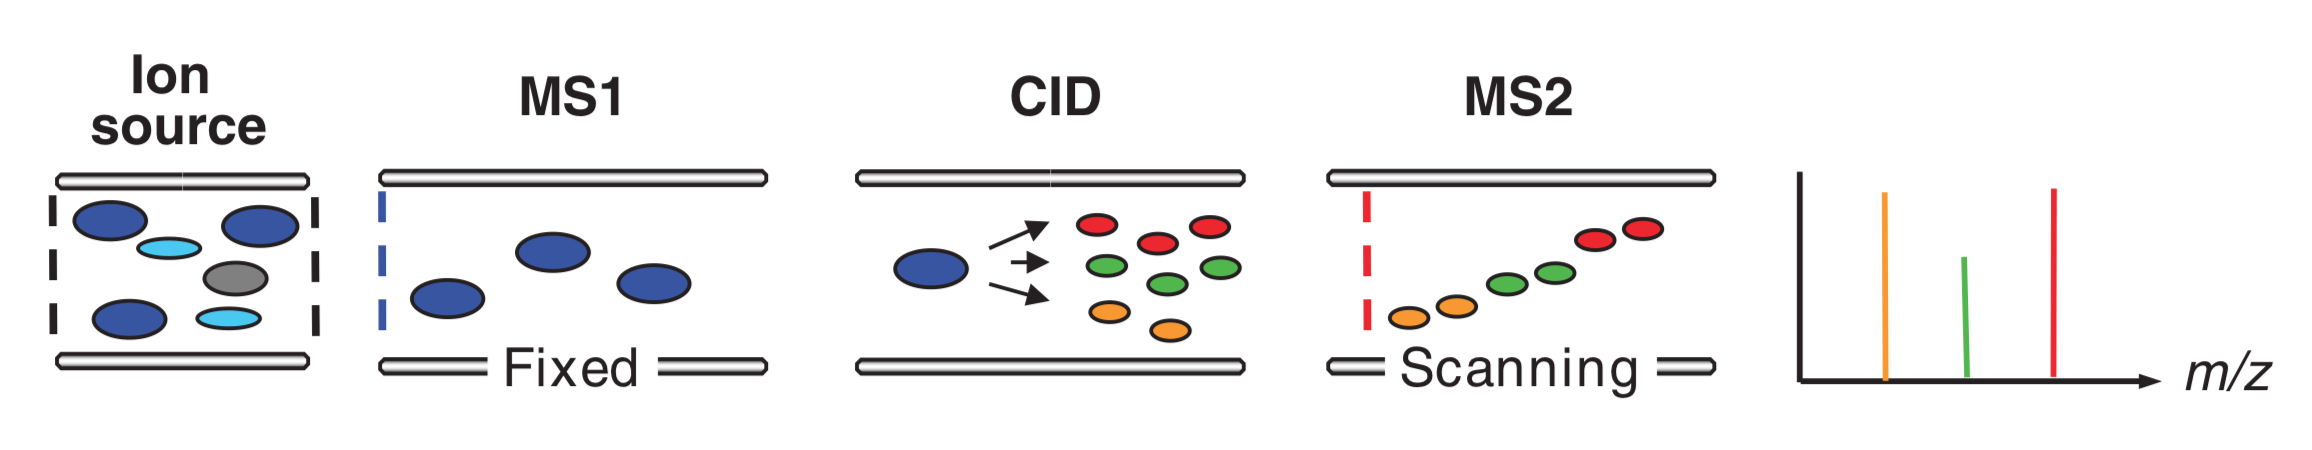
\includegraphics[width=.9\linewidth]{img/msms-workflow.png}
  \caption{A diagram of an ordinary MS/MS workflow. While the specific instrumentation details differ from spectrometer to spectrometer, the general structure of ionize \textrightarrow{} analyse \textrightarrow{} fragment \textrightarrow{} analyse is common to all MS/MS experiments. Image by~\citet{domon2006mass}.}\label{fig:mass-spectrometry-workflow}
\end{figure}

Both the single-stage and MS/MS experiments begin similarly: the sample peptides are ionized (see \Cref{sec:ionisation}), and the ions travel through an electromagnetic field in an analyser whilst their mass-to-charge (\(m/z\)) is being calculated (\Cref{sec:msms-analysis})~\cite{gross2006mass}. In single-stage mass spectrometry, the experiment ends there, while in MS/MS, some of these \emph{precursors} are selected to undergo fragmentation in the collision cell (\Cref{sec:fragmentation}); the typical MS/MS workflow is shown on \Cref{fig:mass-spectrometry-workflow}. The resulting fragments are analysed and their \(m/z\) values noted; the output of the MS/MS experiment is made of precursors with their masses and their fragmentation spectra; an example of a precursor fragmentation spectrum can be seen on figure \Cref{fig:frag-spectrum}.

\begin{figure}
  \centering
  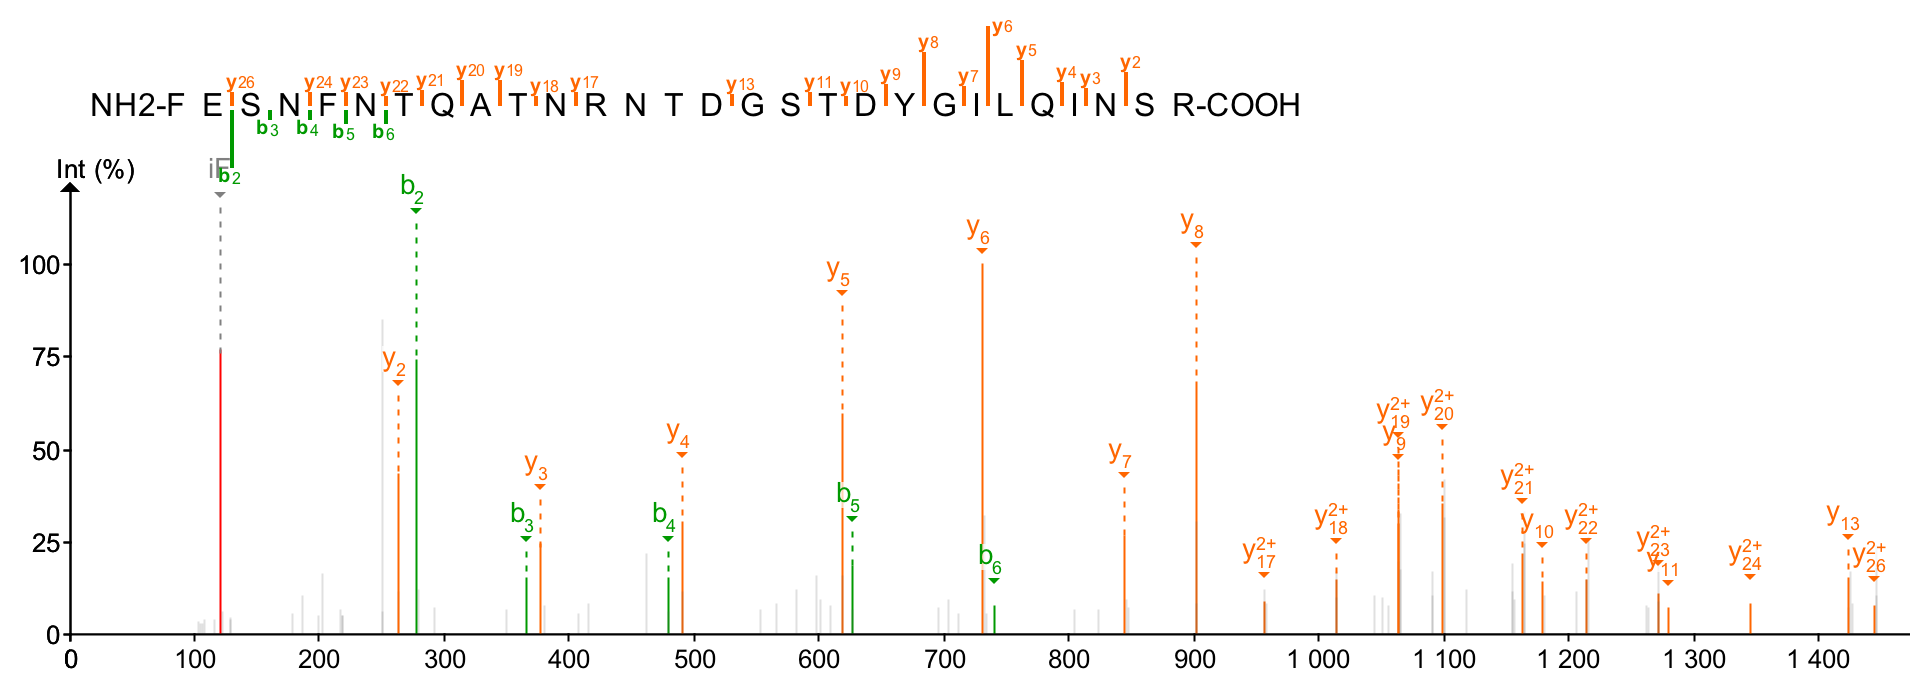
\includegraphics[width=1\linewidth]{img/fragmentation-spectrum.png}
  \caption{An annotated fragmentation spectrum of the precursor \emph{FESNFNTQATNRNTDGSTDYGILQINSR}. A \emph{peak} signifies that a peptide with a specific \(m/z\) value has been seen, and also provides information about the intensity of its signal.}\label{fig:frag-spectrum}
\end{figure}

When the analysed protein is crosslinked by DBs, some of the precursors will be crosslinked, too. The aim of the DB MS/MS analysis is to identify the crosslinked precursors and deduce the positions of DBs in the protein. Specific instrumentation choices influence the behaviour of crosslinked peptides during the analysis, and result in fragmentation spectra with vastly different characteristics. Sometimes one approach is preferable; for example in the case of picking an analyser, orbitrap is usually preferred thanks to its accuracy and sensitivity. Other times the choice is more ambiguous, such as the choice between CID and ETD fragmentation. We discuss the possible intstrumentation choices in the context of DB mapping in the following sections; the overview is partly based on the works of \citet{matthiesen2007mass} and \citet{gross2006mass}.

\subsection{Sample ionization}\label{sec:ionisation}

Only charged compounds in gas phase are detectable by a mass spectrometer analyser. If the samples are not in this form, they need to be ionised.

One of the oldest ionisation methods is electron ionization (EI)~\cite{field2013electron}. However, EI is unsuitable for large thermally unstable organic molecules, such as peptides; for proteomics work, the two most popular options are MALDI and ESI~\cite{caprioli1997molecular, fenn1990electrospray}.\@ Unlike ESI, the MALDI ionisation process has to be done in a vacuum, making it impossible to directly connect a LC column to the spectrometer. Thus, for the purpose of DB mapping, ESI is usually the ionisation method of choice.

During ESI, a very fine capillary with a solution that contains the sample peptides and charged ions is placed into a strong electrostatic field. Due to the influence of the field, the solution forcibly squirts out of the capillary, creating a mist of miniscule charged droplets. The solution slowly evaporates from the droplets, until eventually the repulsive electric forces inside the droplet overcome its surface tension and the droplet splits into yet smaller droplets~\cite{rayleigh1882xx}. This evaporating and splitting process repeats itself, until we are left with isolated sample ions in the gas phase~\cite{dole1968molecular,dole1968gas,fenn1989electrospray, fenn1990electrospray}.

For our work, three properties of ESI are important.

\begin{itemize}
  \item ESI works under atmospheric pressure, enabling the LC colon to be connected directly to the mass spectrometer, creating an ``online'' or ``hyphenated'' LC-MS system~\cite{opiteck1997comprehensive}. This property simplifies the MS/MS experiment and provides higher throughput.
  \item The ionisation cases very little to no fragmentation to the sample~\cite{griffiths2001electrospray} --- in other words, ESI a ``soft'' ionisation technique. This property is useful because it simplifies the subsequent analysis, and does not add noise to the measured information.
  \item  Ions generated by ESI are often multiply charged~\cite{felitsyn2002origin}, bringing their \(m/z\) value down and enabling us to analyse peptides with a higher mass in an ordinary mass spectrometer setting.
\end{itemize}

\subsection{Mass analysers}\label{sec:msms-analysis}

A mass analyser, sometimes equipped with a separate detector, measures the mass to charge ratio (\(m/z\)) and intensity of a sample compound. The many existing mass analysers differ in the principle of function, and their performance characteristics.

\begin{description}
  \item[Time-of-flight analyser] In TOF analysers~\cite{stephens1946pulsed}, sample ions are accelerated with an electric field to make them travel along a path with known length. The ions with lower \(m/z\) values will arrive measurably sooner than the ones with higher \(m/z\) values, as long as all of them are dispersed at a similar-enough points in time. Due to this requirement, TOF analysers are best suited for pulsed ionization techniques such as MALDI\@. TOF analysers have an excellent sensitivity and, at least in theory, their \(m/z\) range is unlimited~\cite{fuerstenau1995molecular}.
  \item[Linear quadrupole analyser] As the name suggest, a linear quadrupole consist of four linear rods which are placed parallel to each other and arranged in a square shape, see \Cref*{fig:quadrupole}. A pair of rods sitting in diagonally opposite corners has the same polarity, however, the pairs periodically switch the polarity. An ion travelling along the rods is periodically repelled and attracted to each of the rods, its precise trajectory depending on its \(m/z\) value~\cite{paul1990electromagnetic}. In this way, ions with specific \(m/z\) values can pass through the quadrupole into a detector~\cite{paul1953neues}, while others follow an unstable trajectory and crash into one of the poles or the wall of the quadrupole.

    Quadrupoles can also trap specific ions inside instead of making them simply pass through; such quadrupole is usually called a linear ion trap~\cite{mao2003h}. Furhtermore, quadrupoles can serve as fragmentation collision cells. Due to their flxibility, a tripple-quadrupole mass spectrometer was a popular choice for MS/MS experiments~\cite{yost1978selected}.
  \item[FT-ICR analyser] In Fourier transform ion cyclotron resonance analysers (FT-ICR) the analytes circulate in a magnetic field, and Fourier transform is used to decode the induced signals. The \(m/z\) values are calculated from the frequencies and amplitudes~\cite{comisarow1974fourier}. Many ions with wildly different \(m/z\) values can be measured in parallel, making the analysis faster. Further improvements also increased the mass accuracy and resolution beyond what is attainable by quadrupole analysers~\cite{amster1996fourier, easterling1999routine}.
  \item[Orbitrap analyser] The Orbitrap is the most imporant analyser type in the context of our work~\cite{hu2005orbitrap}. It achieves similar accuracy, resolving power, and dynamic range to FT-ICR, but does not require an expensive-to-run supraconducting magnet to do so. In Orbitrap the ions simultaneously cycle around the centre and oscillate along the z-axis, as is illustrated on \Cref*{fig:orbitrap}. This oscillation induces a periodically changing electrical current in the detector that is converted to a \(m/z\) spectrum of the analyte with the help of Fourier transform.

    The Orbitrap often achieves sub-ppm error rates, which makes it ideal for our usecase. Our goal is to identify complicated ions, and for that we need the measurements of their mass to be as reliable as possible. Furthermore it is possible to connect Orbitrap to an ESI ion source, and by extension to a LC colon.
\end{description}

\begin{figure}
  \centering
  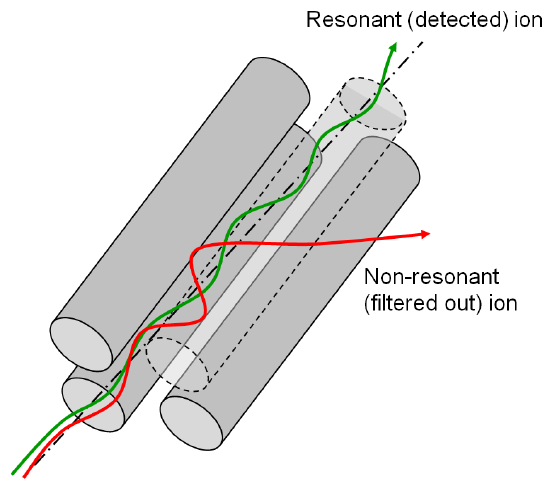
\includegraphics[width=.4\linewidth]{img/quadrupole.png}
  \caption{A quadrupole with two highlighted classes of ion trajectories. Thanks to its \(m/z\) value, the ion with green trajectory passes through the quadrupole and is ultimately detected, while the one with the red trajectory is filtered out. Image taken from~\citet{2021Mass}.}\label{fig:quadrupole}
\end{figure}

\begin{figure}
  \centering
  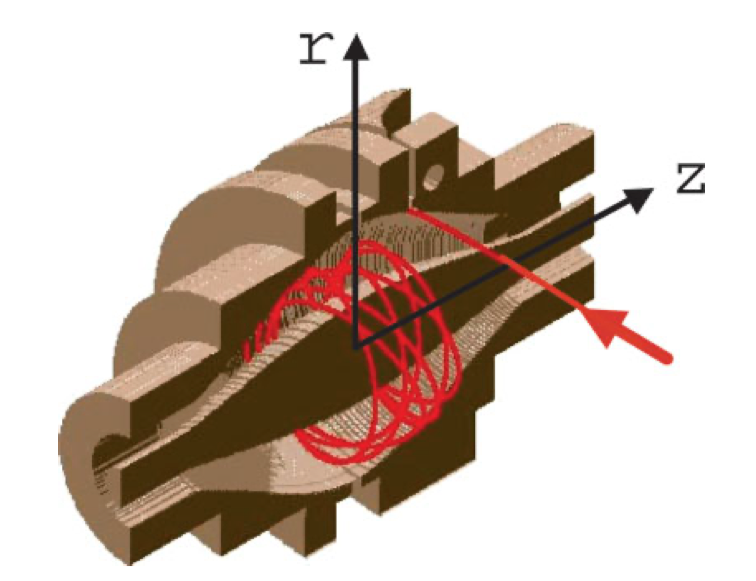
\includegraphics[width=.5\linewidth]{img/orbitrap.png}
  \caption{An Orbitrap mass analyser with a typical ion trajetrory highlighted. The ion circulates around the center while simultanously oscillating along the z-axis. Image by~\citet{hu2005orbitrap}.}\label{fig:orbitrap}
\end{figure}

\subsection{Precursor fragmentation}\label{sec:fragmentation}

In MS/MS experiments, once the mass spectrum of the initial sample is analysed and the MS\textsuperscript{1} data are acquired, \emph{precursors} are selected according to their mass, and fragmented. The fragments undergo yet another mass analysis, producing so called MS\textsuperscript{2} data. In the section we present a short overview of the currently used fragmentation methods.

When the goal of the experiment is to observe post-translational modifications (PTMs) and to preserve the volatile bond connecting the PTM to the peptide, electron-capture dissociation (ECD)~\cite{zubarev2000electron} or electron-transfer dissociation (ETM)~\cite{syka2004peptide} are preferred. Both methods use electron transfer to induce amine backbone bond cleavage that results in the creation of \(c\) and \(z\) ions, as illustrated on \Cref{fig:fragment-types}.

During ETD, the DBs are dissociated, and the crosslinked precursor is split into its constituent peptides~\cite{liu2014facilitating}. These peptides appear as high-intensity peaks in the fragmentation spectra. The peaks which can be used to determine the peptide makeup of the orignal precursor, which causes ETD to be a popular fragmentation technique in DB mapping methods. However, if the precursor contains multiple cysteines, it may be hard to deduce which of them were paired together, especially if there were multiple DBs present. In this work we focus on methods that do not have this disadvantage.

First of these methods is collision-induced dissociation (CID). CID accelerates the precursor ions, and makes them collide with neutral gas molecules, ultimately leading to their fragmentation. The dissociation process usually takes place at the more labile bonds, such as the ones connecting PTMs~\cite{quan2013cid}, or peptide bonds in the precursor backbone.\footnote{The fact that many PTM bonds are preferentially dissociated during CID is usually seen as unfortunate. However, in the case of DB mapping it simplifies the analysis, as the PTMs can be safely ignored, which reduces the combinatorial complexity of the problem.} CID produces \(b\) and \(y\) fragment ions (see \Cref{fig:fragment-types}); additionally, as a side-effect of the dissociation, a small neutral molecule sometimes breaks off of the fragment, lowering its total mass value without affecting its charge. This dissociated molecule is called a \emph{neutral loss}. In CID, the most common neutral losses are water and amonia.

A specific variant of CID called the beam-type CID produces \emph{internal ions}, fragments that are generated by two (or more) bond cleavages during the fragmentation. Many of the internal ions begin with a proline~\cite{michalski2012systematic}, suggesting that the double cleavage event prefers some amino acids to others. As shown by \citet{michalski2012systematic}, ion-trap CID, the other CID variant, does not produce internal ions. Furthermore, ion-trap CID has limits regarding the containment of molecules below a certain mass threshold, leading to a mass cutoff~\cite{louris1987instrumentation}.

\begin{figure}
  \centering
  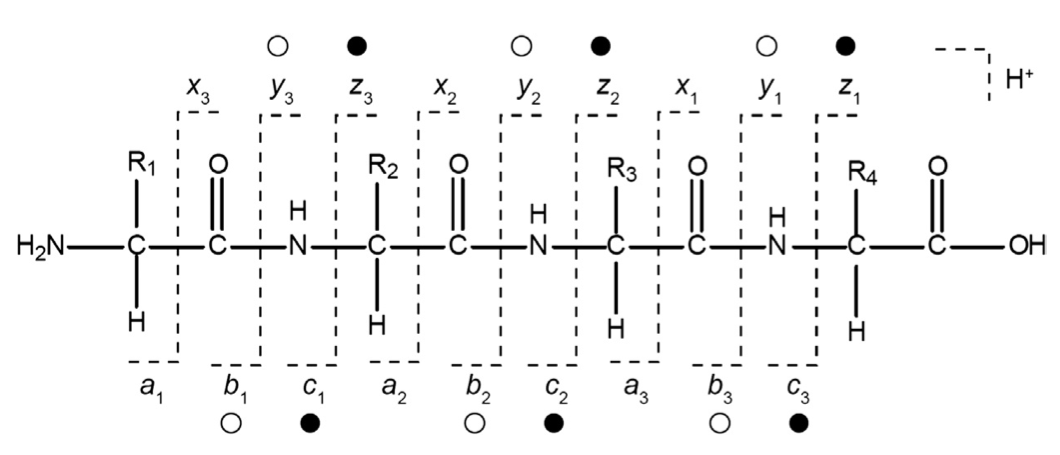
\includegraphics[width=.75\linewidth]{img/fragment-types.png}
  \caption{A singly positively charged peptide with annotated fragmentation types. Signature CID b/y ion fragments are marked with open circles, while the typical ECD and ETD c/z ion fragments are marked with filled circles. Image by~\citet{hart2014review}.}\label{fig:fragment-types}
\end{figure}

A similar fragmentation signature to CID can also be obtained by infrared multiphoton dissociation (IRMPD)~\cite{oomens2006gas}. Because IRMPD, and the related UV-MPD, do not require collision gasses to be present for the fragmentaion, they are well suited for analysers operating under high vacuum, such as FT-ICR\@.

In 2007 a new fragmentation method based on beam-type CID has been devised, called the higher-energy C-trap dissociation (HCD)\@. The fragmentation spectra obtained from CID and HCD are very similar~\cite{michalski2012systematic}, nonetheless there is a key difference between the two methods: HCD combines the richer sequence information~\cite{xia2006ion} and lower mass cutoff of beam-type CID with the superior resolution capacity and accuracy of the orbitrap analyser. That is one of the reasons the data we use in this thesis come from HCD\@. In the next section we describe the common HCD fragmentation pathways, because they are crucial to the function of our DB mapping program.

\subsubsection{Fragmentation pathways in HCD}

Fragments from ESI-ionized precursors can be and indeed often are multiply charged~\cite{katta1991use, michalski2012systematic}. According to the research on CID of crosslinked peptides by \citet{giese2016study}, most of the crosslinked fragments were found to have a positive charge of at least 2, while an overwhelming majority of linear fragments had a positive charge of 1. HCD is in principle similar to CID, and we believe these findings woud translate to HCD-generated fragments as well.

The different types of fragments of a very pure sample were nicely summarized by \citet{michalski2012systematic}. Ions of \(b\), \(y\) and \(a\) type comprise most of the spectral intensity (54\%, see \Cref{fig:hcd}). The ions themselves have different distributions, the \(y\) type being the most abundant. Other neutral loss ions, be it a loss of water, amonia, or an amino-acid-specific small molecule\footnote{If specific amino acid neutral losses are of interest, the review by~\citet{paizs2005fragmentation} lists many of them.}, together with internal ions, can be attributed a quarter of the total fragment intensity. Finally, immonium ions account for 6\% of the intensity. In total 85\% of the spectral intensity is explainable. For a visual overview of the many different HCD fragmentation types, please refer to \Cref{fig:fragment-types-hcd}.

\begin{figure}
  \centering
  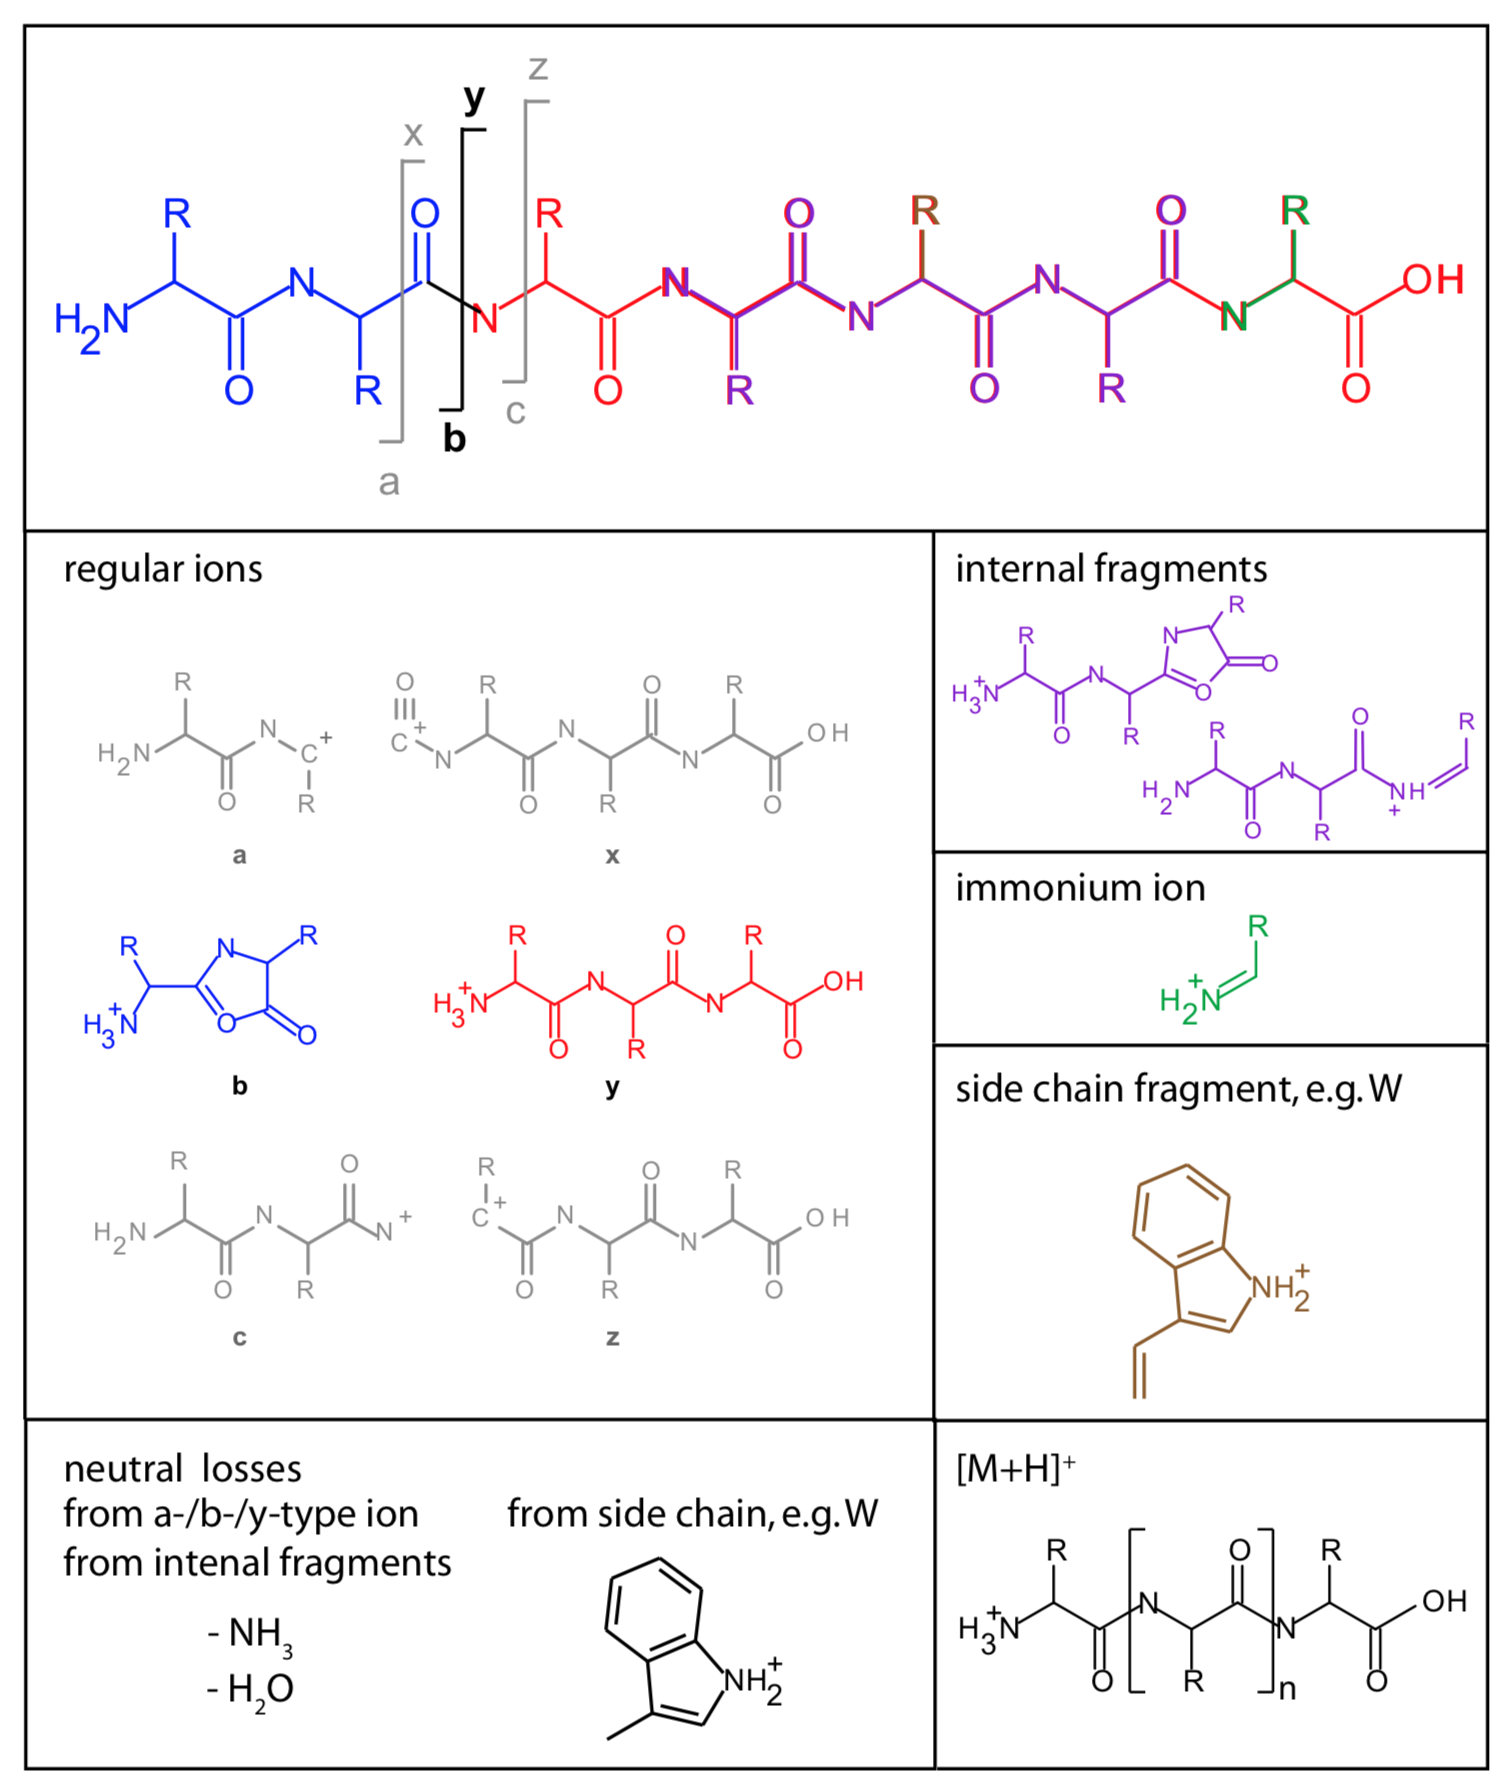
\includegraphics[width=.9\linewidth]{img/fragment-types-hcd.png}
  \caption{During HCD, \(b, y\), and to a lesser extent \(a\), ions are the most common, together with internal ions and immonium ions, and their counterparts with neutral losses. Image by~\citet{michalski2012systematic}.}\label{fig:fragment-types-hcd}
\end{figure}

\begin{figure}
  \centering
  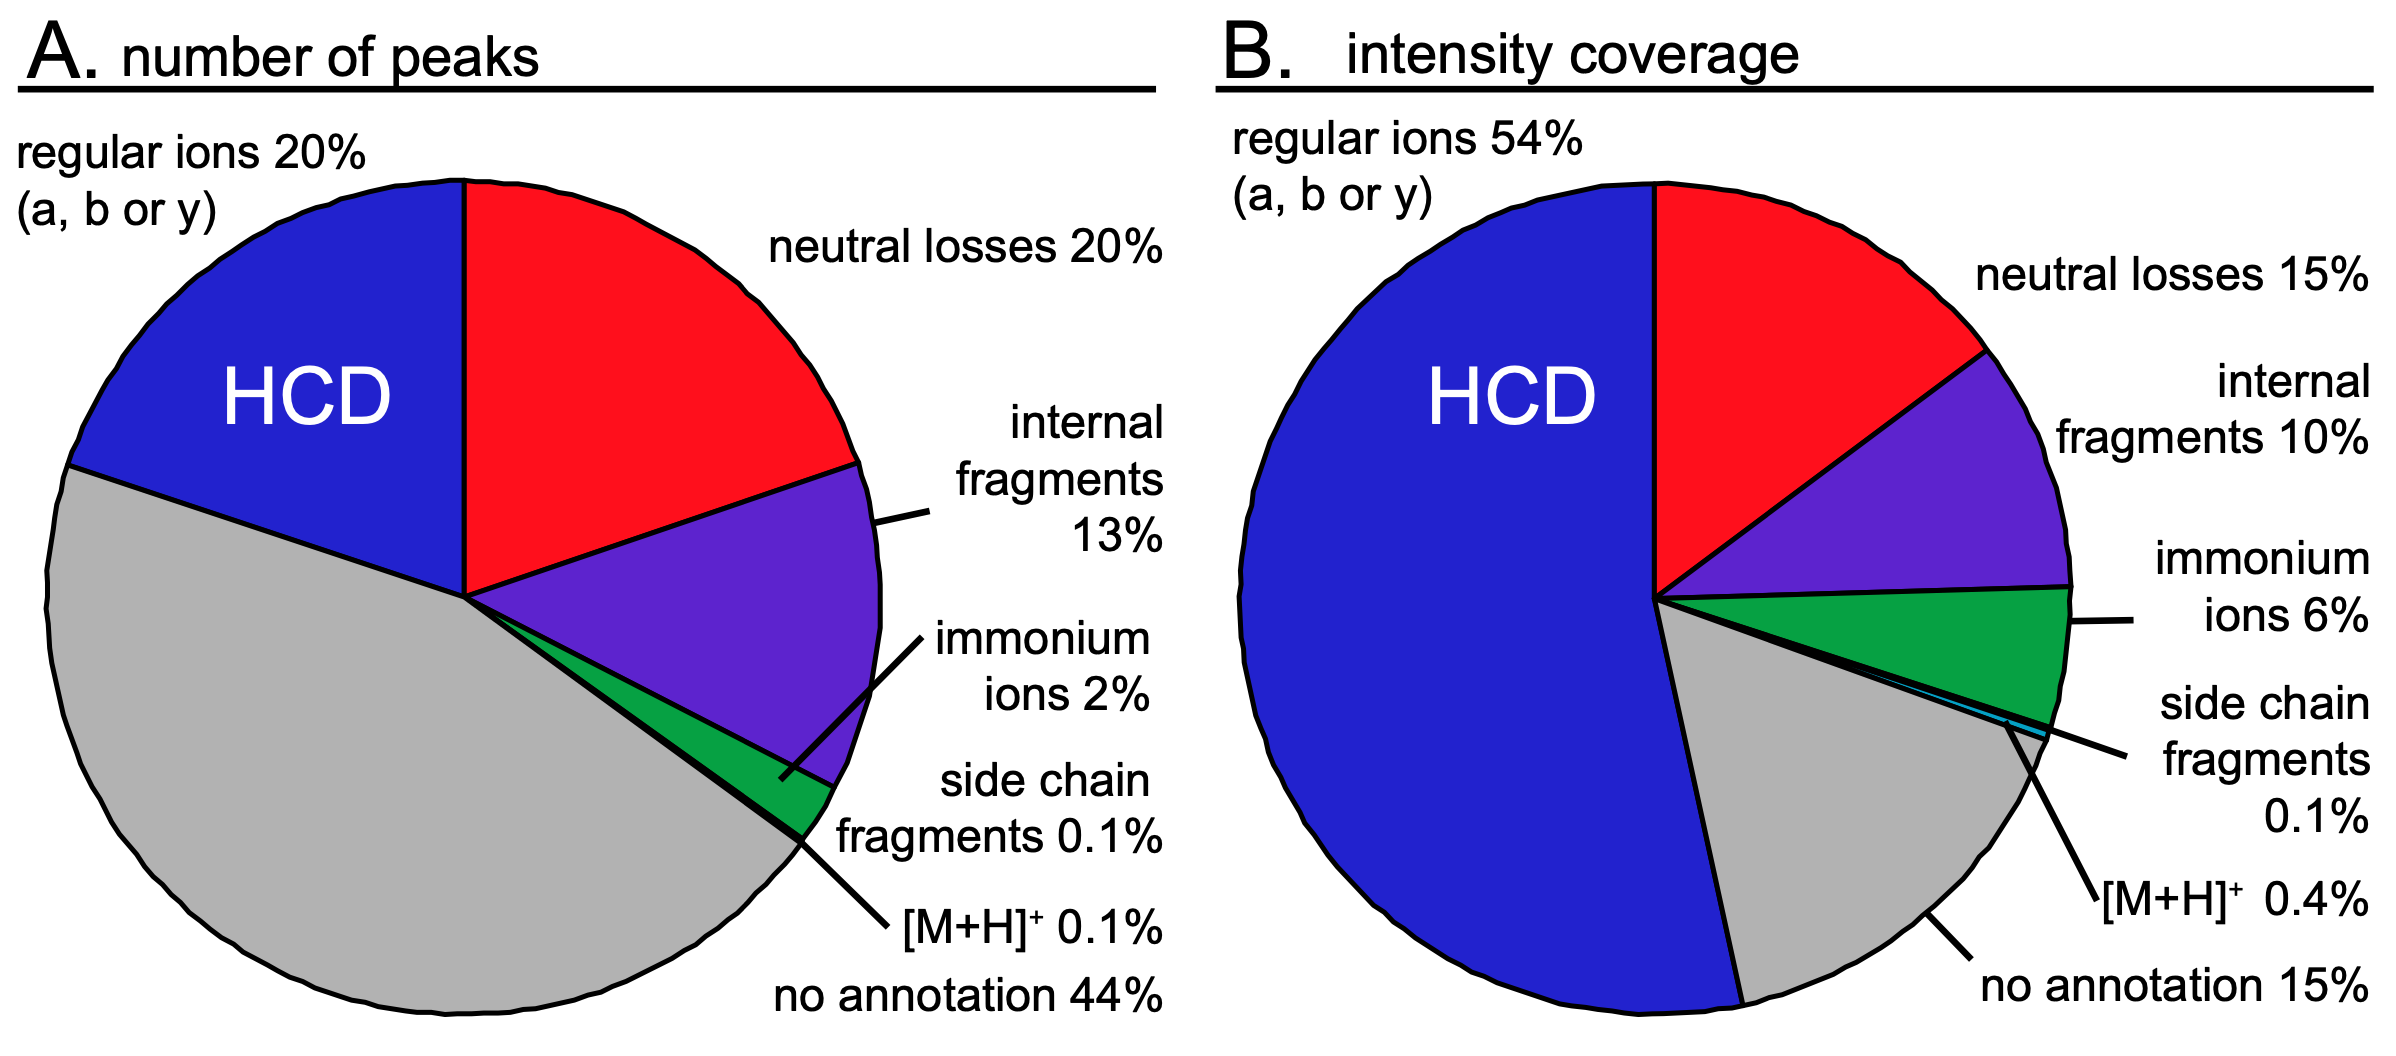
\includegraphics[width=.9\linewidth]{img/hcd.png}
  \caption{(B) The regular \(b, y\), and \(a\) ions take up 54\% of the measured spectral intensity. Another 25\% is explained by fragments with neutral-loss and internal fragments, and another 6\% by immonium ions. Together, those four account for 85\% of the measured intensity. It is true that almost a half of the peaks are still left unexplained (A), however, given all of these fragments have to split the remaining 15\% of intensity, they are probably rather rare and are only of moderate importance. Image by~\citet{michalski2012systematic}.}\label{fig:hcd}
\end{figure}

Although DBs are not affected by low-energy CID as much as the other PTMs~\cite{paizs2005fragmentation, lioe2007novel}, in high energy collision fragmentation such as HCD, cleavage of the S-S bond can be observed with a higher probability~\cite{bean1992characterization}. The cleavage of the bond can result in the formation of an asymetrical distribution of mass on the two cysteines~\cite{zhang2006mapping}, see \Cref{fig:disulfide-bond-cleavage-assymetry} for details. Additionally, the sole presence of a DB influences the fragmentation pathways of the whole peptide; \citet{mormann2008fragmentation} reports a low but detectable signal of peptide backbone cleavages in the bonds instide S-S loop of an internal DB, while \citet{clark2011collision} reports a higher frequence of internal ions.

\begin{figure}
  \centering
  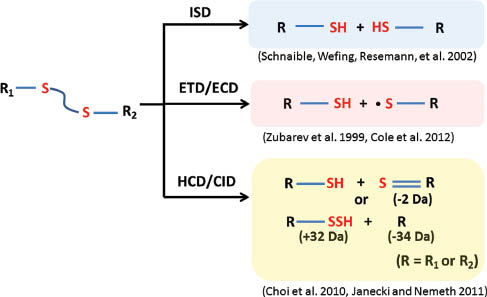
\includegraphics[width=.6\linewidth]{img/disulfide-bond-cleavage-assymetry.jpg}
  \caption{Under different dissociation strategies, DBs manifest different cleavage characteristics. Under CID, the cleavage results into two possible assymetrical mass distributions. Image by~\citet{tsai2013mass}.}\label{fig:disulfide-bond-cleavage-assymetry}
\end{figure}

To recapitulate, in theory a \(b\), \(y\), \(a\), or an internal ion can be seen in a HCD fragmentation spectra with zero or more of the following modifications:

\begin{enumerate}
  \item Dissociated neutral loss.
  \item Covalent modifications on some of the amino acid residues, such as methionine oxidation. A subset of these are the cysteine alkylations.
  \item A piece of a former DB that has been cleaved during the fragmentation.
  \item One or more fragments, possibly modified with some of the above, connected by a set of DBs. For some examples of crossliked fragments, see \Cref{fig:intrapeptide-bonds}.
\end{enumerate}

\begin{figure}
  \centering
  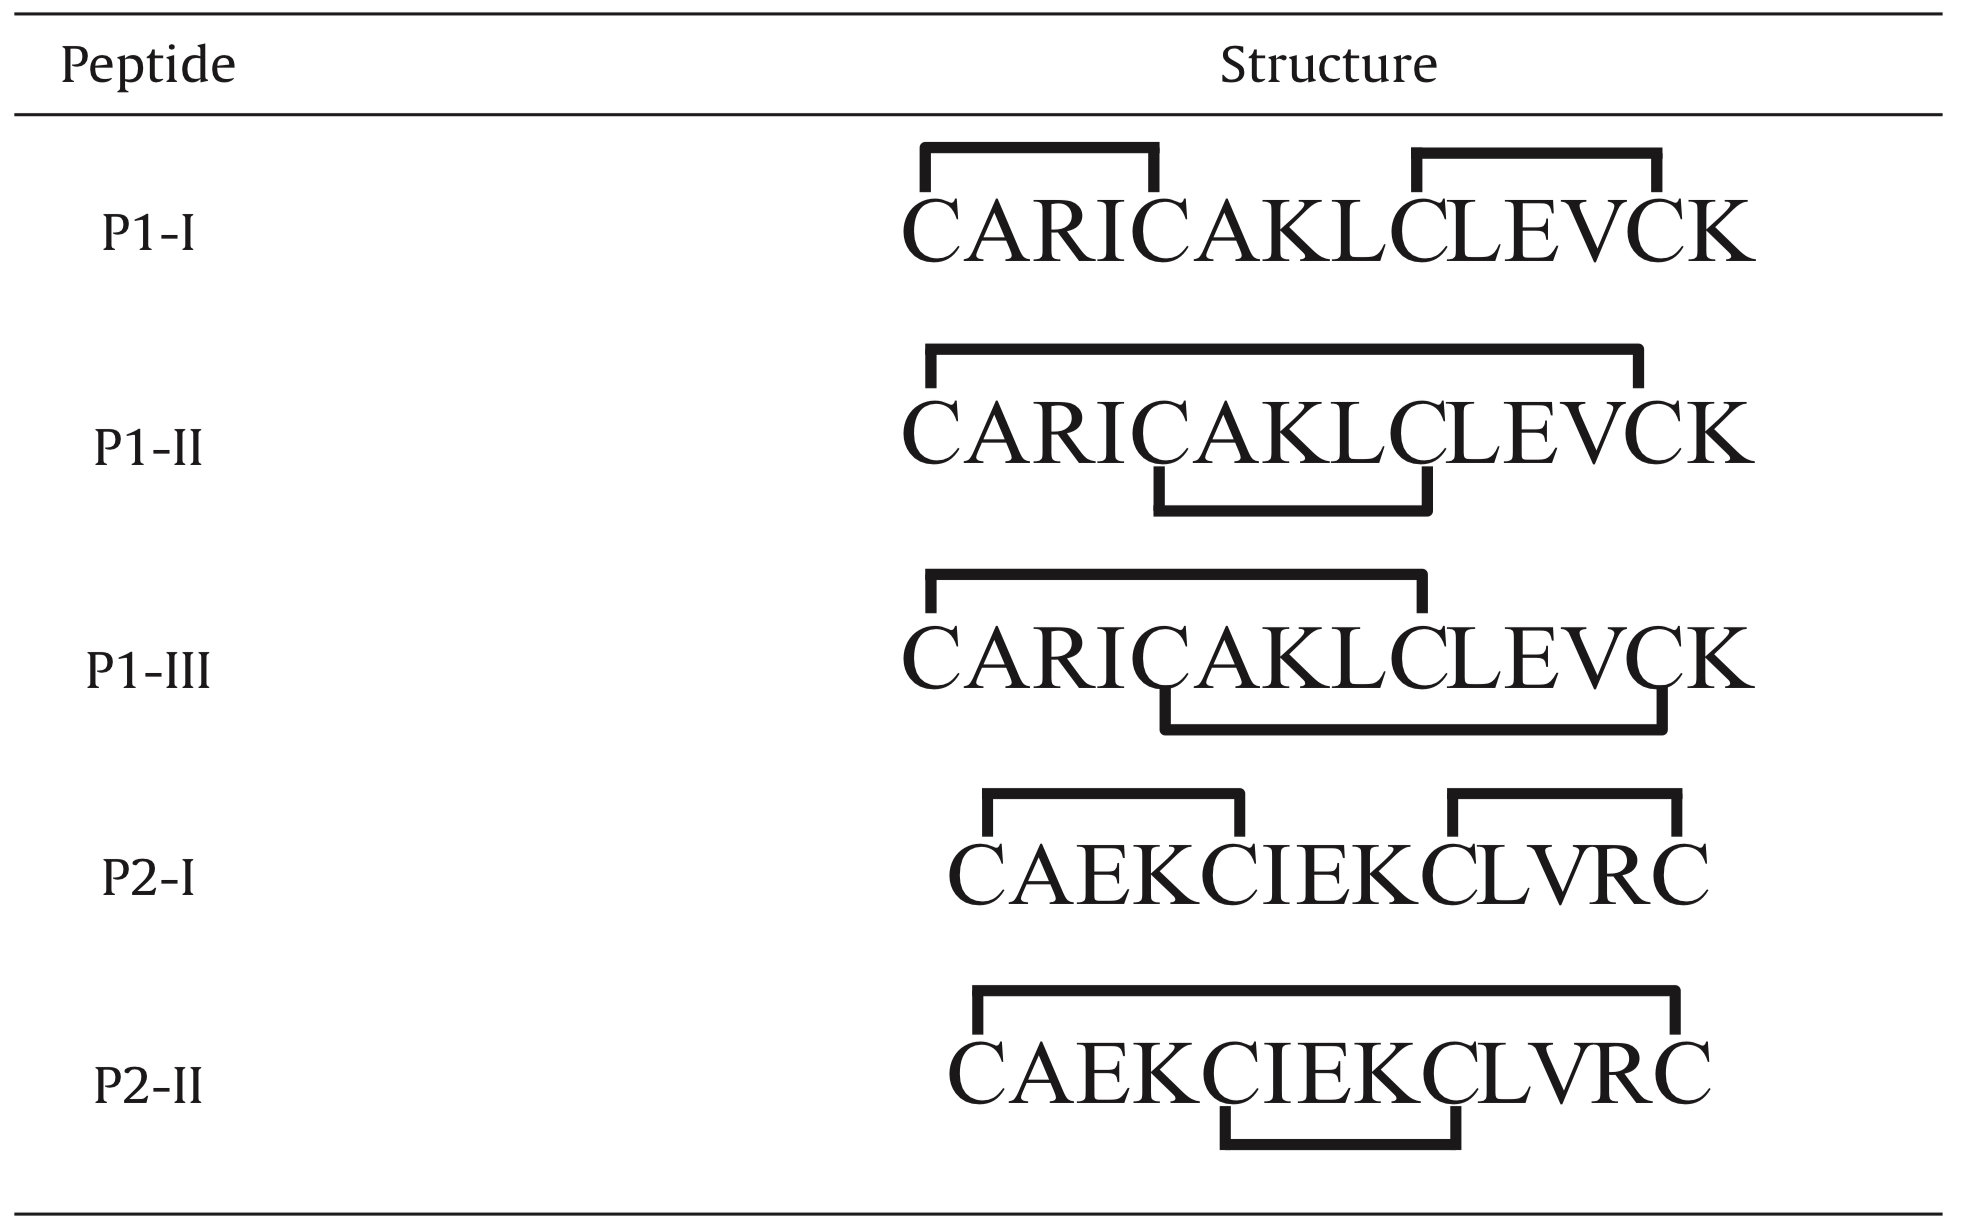
\includegraphics[width=.5\linewidth]{img/intrapeptide-bond.jpeg}
  \caption{An example of different possible configurations of intra-peptide DBs. Image by~\citet{durand2013tandem}.}\label{fig:intrapeptide-bonds}
\end{figure}

If we managed to identify the crosslinked fragments (category 4) in the measured data, we would gain a lot of important evidence about the presence of certain DBs in the protein. However, due to the complexity of the potential fragments, the fragment identification proces is very hard to automate completely. The next section details some of the current approaches to fragment assignment and DB mapping.

\section{Interpretation of fragmentation spectra from crosslinked peptides}\label{sec:analysis}

This section concerns itself with the existing methods that aim to determine the position of DBs in a protein using MS/MS data. After a short review of the manual and computation approaches to this problem, we formulate the task that this thesis is trying to solve in more precise terms, and finally perform a simple complexity analysis of the problem.

As noted by \citet{lakbub2018recent}, there are two main types of DB characterization.

\begin{itemize}
  \item Profile comparison methods make use of two samples: one reduced with the DBs removed, and one nonreduced whose DBs are still intact. Differential analysis is then deployed on a chromatogram profile of these two samples to determine which peptides are in the nonreduced sample, but not in the reduced one. Those peptides are suspect of containing DBs and are further analyzed in MS/MS\@.
  \item Intact analysis methods only use data from the nonreduced sample. Thus, they are simpler from the sample preparation standpoint, but have less information at their disposal than the profile comparison methods.
\end{itemize}

In each of the both categories, the protocols further differ in the choice of of sample separation, ionization, and fragmentation methods, the choice of mass analyzer, and whether the bulk of the analysis is performed manually or automatically~\cite{lakbub2018recent}. Some of the software for automatic DB characterisation is reviewd below; for the sake of completness, an example of a partially-manual method now follows.

\citet{wu2009mass} propose an intact analysis method based on LC-MS/MS with ETD\@. The prepared peptides are measured on MS\textsuperscript{1}, and fragmented by ETD\@. As described earlier, if the precursor ion contains DBs, they are dissociated in ETD, resulting in fragmentation spectra with two prominent peaks. The two peaks represent the two peptides that were connected by a DB to become the original precursor ion. Fragments from these two peaks are put into an MS\textsuperscript{3} step that employs CID fragmentation to acquire their sequence information. This sidesteps the problem of not having data from the non-bound peptides in the intact methods. Software for fragment mass searching and matching is used, but because it is not made with DB research in mind, the method requires frequent manual interventions.

It is clear that using specialised software for DB mapping would be preferable in this scenario. We reviewed some of the current computational methods in the next section.

\subsection{Current computational approaches}

Dedicated DB characterisation software usually only needs data from nonreduced samples. Nonetheless there are some commercial options that offer the possibility to add data from reduced samples, too, such as PepFinder and BioPharma Finder, as noted by \citet{lakbub2018recent}. The same authors offer a comprehensive list of past and current manual and compuational DB characterisation methods.

SimXL is tool for general peptide cross-linking analysis~\cite{lima2015sim}, including DBs~\cite{cui2019comprehensive}. SimXL has three main differentiating factors. Frist is the user-friendly UI that allows the reasearchers to view not only the interpreted results, but also the annotated data based on which they were computed. Second is its search space reduction heuristic based on the presence of a reporter ion~\cite{iglesias2010identification}, a peak that is specific to the fragmentation spectra of a crosslinked precursor. Finally, SimXL employs a further search space-reduction heuristic based on dead-end modifications, but we believe it is probably inapplicable in the context of DB characterisation.

A popular method by \citet{liu2014facilitating} includes a recommened research protocol, starting with protein digestion. Samples are digested with pepsin to avoid DB scrambling, fragmented with ETD followed by HCD, or (EThcD) for short, and finally analyzed with SlinkS, a dedicated DB matching algorithm. As mentioned previously, it is possible to extract information about the peptides constituting the precursor ion from the ETD fragmentation spectra. The HCD step is employed in order to gain sequence information about these peptides, similary to how MS\textsuperscript{3} has been used in~\cite{wu2009mass}.

Ultimately, thanks to EThcD, two peaks corresponding to the precursor peptide pair are identified in each fragmentation spectrum. Aditionally, the whole precursor match is scored by scoring the fragments, now that it is known from which precursor they (allegedly) originated. The main shortcoming of this method is the fact that it only works with dipeptide precursors connected by a single DB; it also ignores fragments with neutral loss and internal ion fragments. That makes it impossible to identify some of the more complicated DB configurations, such as the ones on \Cref{fig:intrapeptide-bonds}.

In fact, all of the aforemetioned methods should be able to match simple interpeptide DBs, but they reportedly struggle with more complex DB configurations~\cite{lakbub2018recent}; for some examples of complicated DB configurations, see \Cref{fig:bond-types}.

A wide array of approaches to DBs is offered, leading to a yet wider array of recommended sample preparation and fragmentaion protocols. We conclude that computational DB characterisation is a hard problem to solve, a notion we formalize in the next section.

\begin{figure}
  \centering
  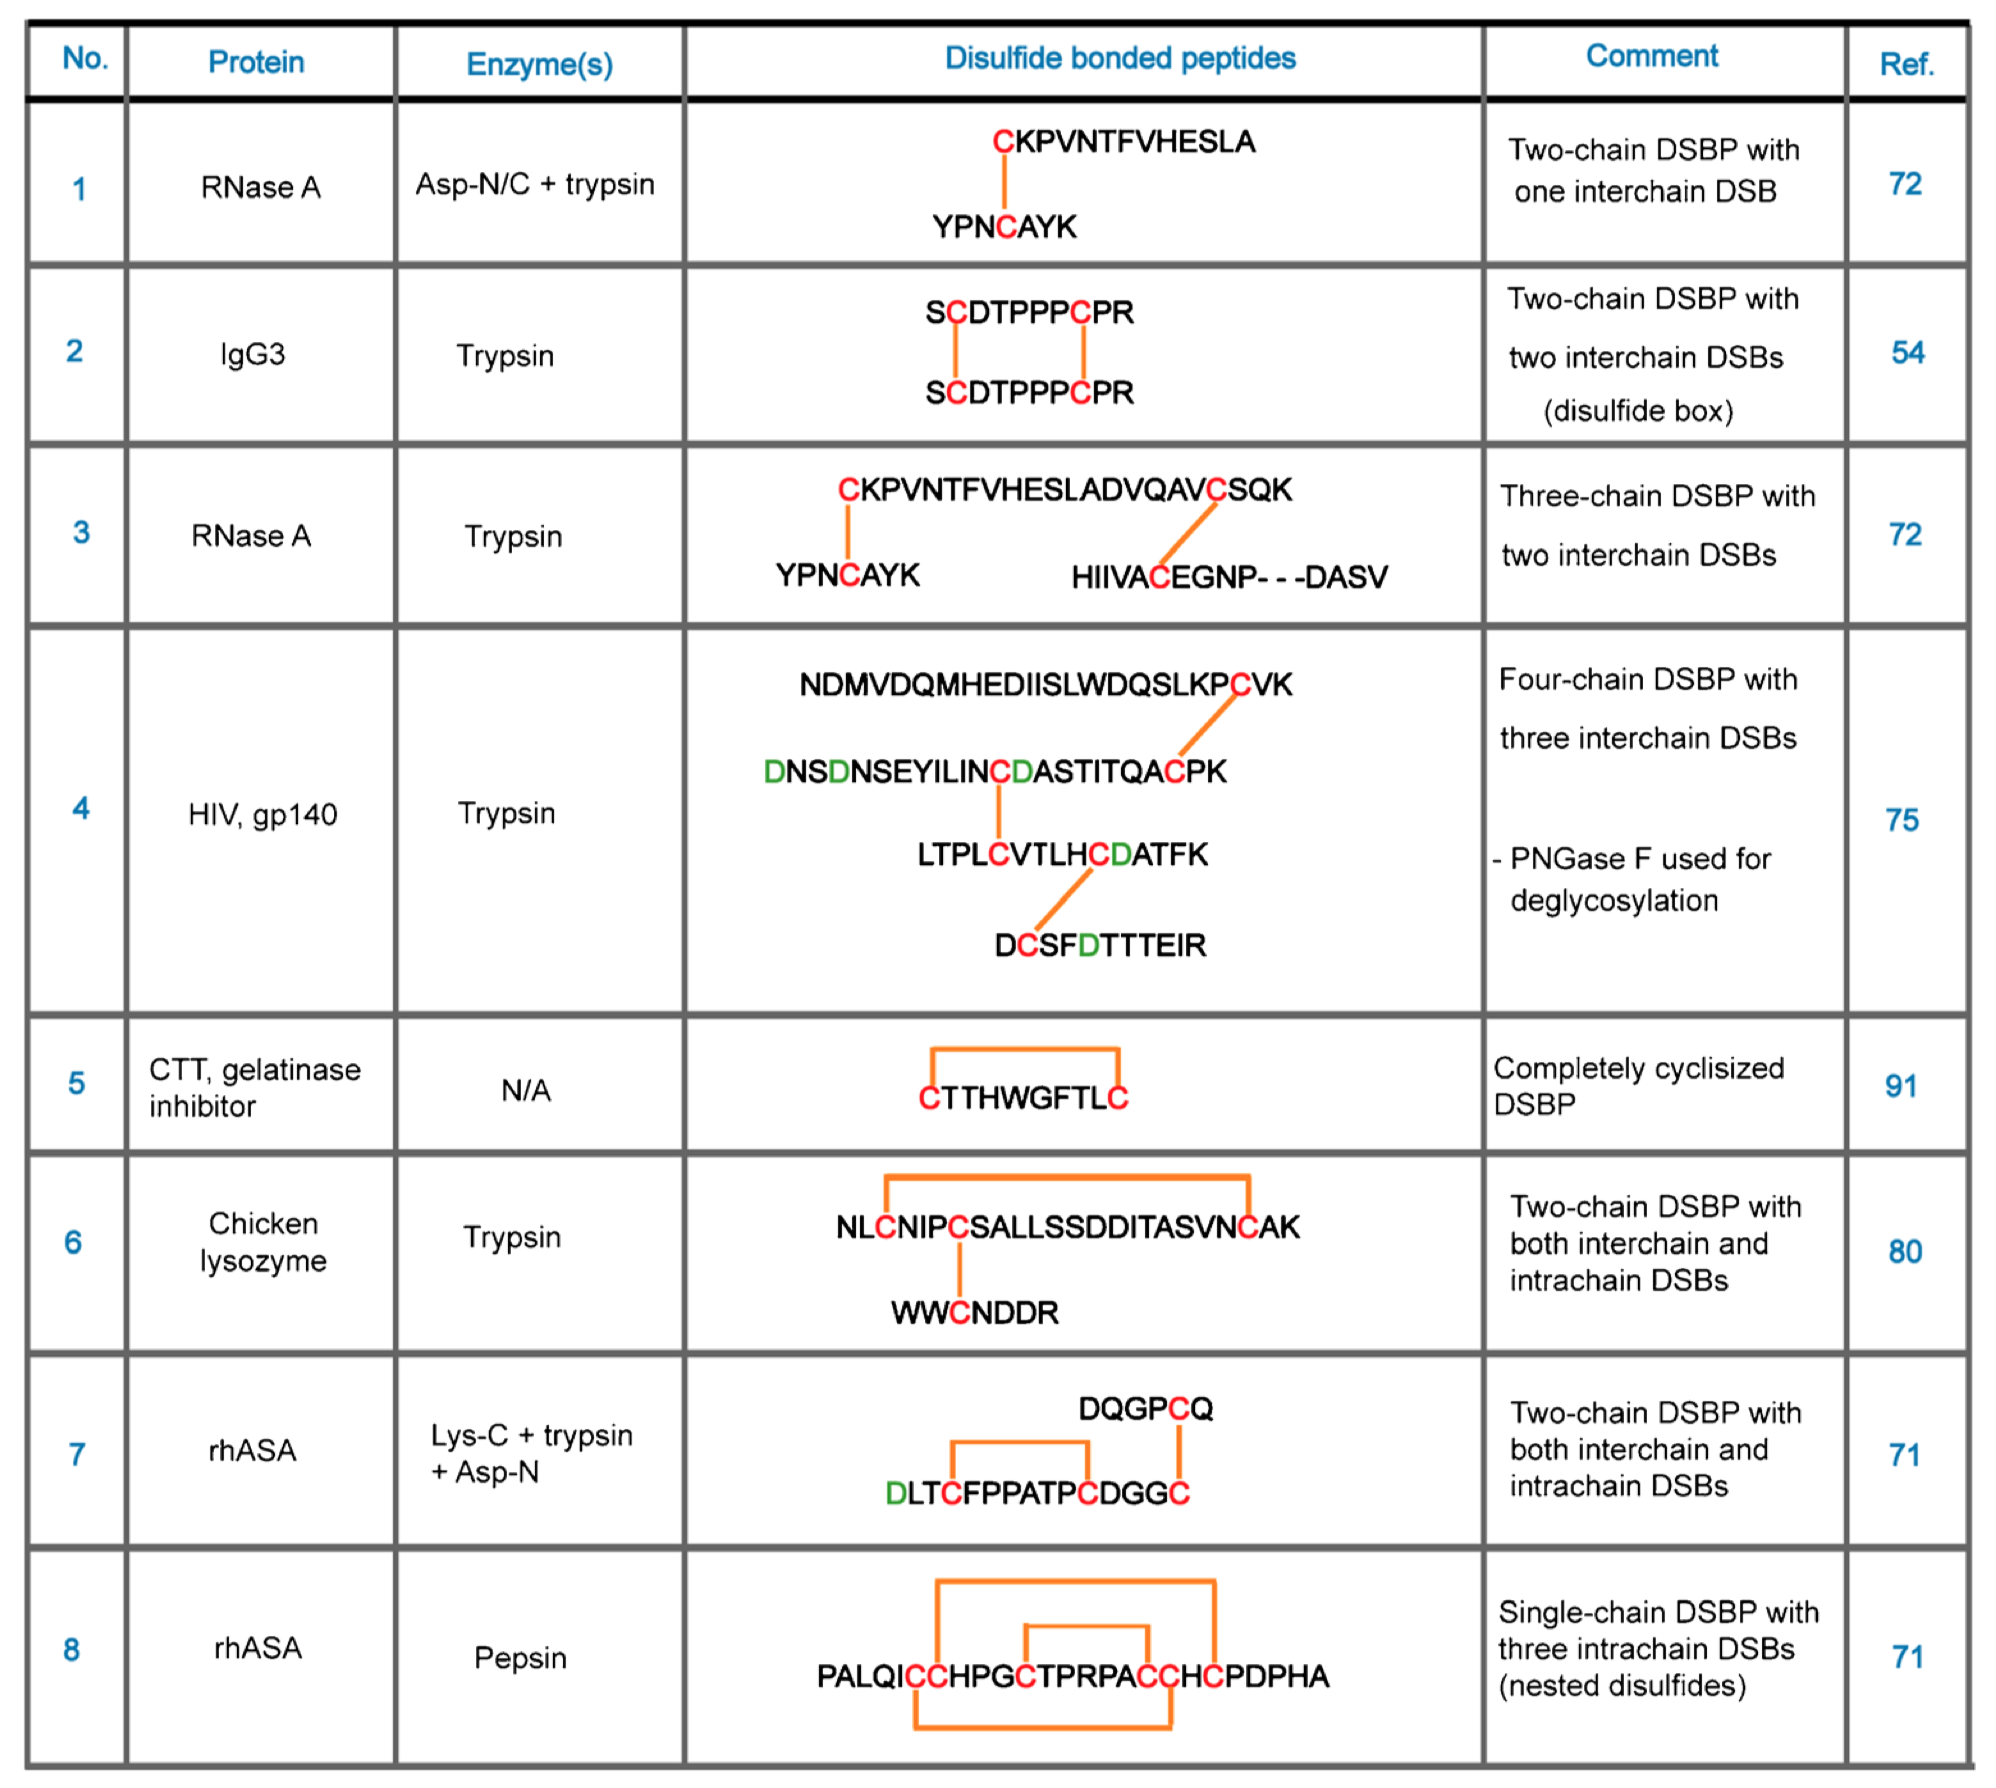
\includegraphics[width=1\linewidth]{img/bond-types.png}
  \caption{Illustrative examles of different ways peptides can be connected by disulfide bonds, ranging from realtively simple examples (1, 3, 5) to complex multipeptide or multibond configurations (4, 8). The more complicated configurations proved to be hard to characterise computationally. Image by~\citet{lakbub2018recent}. (DSB = disulfide bond, gp140 = glycoprotein 140, rhASA = recombinant human arylsulfatase A)}\label{fig:bond-types}
\end{figure}


\subsection{Computational complexity of crosslinked fragment identification}

Undisputably, the problem of determining the characteristics of DB linkages in proteins is hard. From biochemical point of view, already sample preparation poses a challenge; there is a need to minimize DB scrambling, but at the same time have the protease be as specific as possible to simplify the subseqeucnt analysis.

Another unresolved problem is the choice of dissociation method. ETD spectra offer the information about the constituent peptides, which is useful when assigning precursor peptides. On the other hand, CID-based approaches have access to richer but more complicated fragmentation spectra, including interlinked fragments and internal ions with intact DBs; these are useful for precise pinpointing of the DB location.

To continue this discussion further, we need to be specific about the precise task we are attempting to solve. The ultimate goal is to determine where all DBs in a protein are located, even if they are in complex configurations. In this thesis, we try to reach this goal by identifying a wide array of fragments in the measured fragmentation spectra, and aggregating the evidence they provide about positions of the individual DBs. So, to solve the original DB mapping problem, we need to be able to identify even complex fragments in MS/MS data.

\subsubsection{A formalised perspective of the task}

We have a known precursor with defined DB positions, that we will call a \emph{variant}, and a measured fragmentation spectrum. Our task is to say how well the variant matches the spectrum, by trying to assign in-silico generated fragments of the variant to the different measured peaks. Mathematically, we can represent the variant by a \emph{variant graph}.

\begin{defn}
  A \emph{variant graph} of a variant \(R\) comprising of \(n\) residues is a graph \(G_R = (V, E)\) with weighted nodes, where \(V  = 1\ldots n\) and \((i, j) \in E\) if and only if there is a peptide or a disulfide bond connecting  the \(i\)-th and \(j\)-th residue in \(R\). The weight \(w_i\) of the vertex \(i\) is the mass of the corresponding \(i\)-th residue in the precursor.
\end{defn}

Even though the bonds in \(R\) are constrained in terms of connectivity --- there can be at most one DB connected to a given residue, and at most two peptide bonds --- \(G_R\) can still in theory be a relatively complex non-planar graph, as illustrated on \Cref{fig:nonplanar}.

\begin{figure}
  \centering
  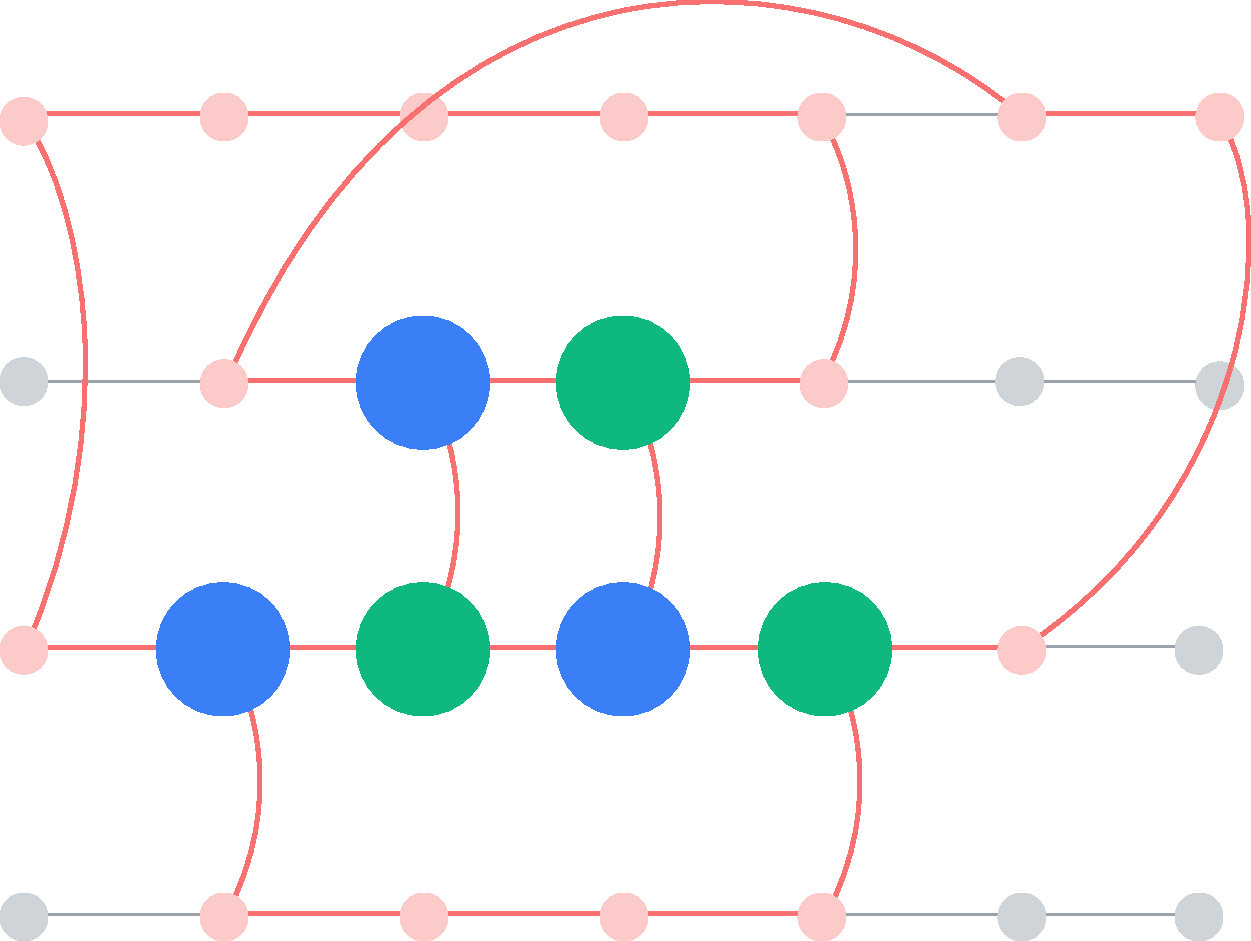
\includegraphics[width=0.5\linewidth]{img/nonplanar.pdf}
  \caption{An example of a valid precursor graph that is not planar due to the presence of a \(K_{3, 3}\) subdivision~\cite{kuratowski1930probleme} (highlighted). Vertices represent amino acid residues, horizontal lines represent peptide bonds, and vertical curved lines represent disulfide bonds. The precursor could be made out of four different interlinked peptides, but it is alsopossible for it to be a single peptide with many intrapeptide disulfide bonds.}\label{fig:nonplanar}
\end{figure}

\begin{lemma}\label{lemma:fragment}
  Every fragment \(A\) of the variant \(R\) can be represented as a connected weighted subgraph in \(G_R\), and every connected subgraph in \(G_R\) represents a fragment of \(R\). We will denote the connected subgraph represeting the fragment \(A\) as \(F_A\).
\end{lemma}

\begin{lemma}\label{lemma:mass}
  The number of cleavages that were required to create the fragment \(A\) is equal to the number of edges that have at least one vertex in \(F_A\), but are not themselves in its set of edges. The mass of \(A\) can be computed by summing up the weights of its vertices \(F_A\).
\end{lemma}

The task of matching the whole variant to a spectrum can be split into multiple subtasks of trying to find a fragment of the variant that matches a mass of a specific peak. By using \Cref{lemma:fragment} and \Cref{lemma:mass} we can reformulate the subtask as searching for a connected subgraph in \(G_R\) in which the sum of vertex weights is equal to the mass of the peak we are trying to match. This problem is usually called the exact weight subraph problem~\cite{abboud2013exact}, or, in our case, an exact weight \emph{connected} subgraph problem.

A well-studied closely related problem called the maximum weight connected k-subgraph problem was shown to be NP-hard on general graphs, and even on planar and bipartite graphs with integer weights~\cite{hochbaum1994node}.\footnote{The same authors propose a polynomial-time \(O(k^2n)\) dynamic programming algorithm for a restricted version of the problem searching for subgraphs in trees.} The exact weight connected subgraph problem has not been studied quite as thoroughly, but we believe it is safe to assume that its complexity will not be much lower. In other words, in the context of our not-necessarily-planar precursor graphs, the problem is likely NP-hard.

Furthermore, this was only a simplified look on the fragment matching problem. In reality, we are not looking for an exact match, but we have a tolerance range whose size is not absolute, but is defined relative to the mass of the generated fragment (in ppm). We also have to take into account the possible modifications of amino acid residues, the possibile occurences of a neutral loss, and the asymetrical nature of disulfide bond cleavage under CID, adding additional complexity to an already complex problem.

Nevertheless, in the next chapter we describe a general algorithm that attempts to solve the fragment matching problem, and use the results to identify DBs in the original protein. We apply an upper bound on the number of cleavages of matched fragments, which limits the search space considerably. We also employ strict limits regarding the matching error, which enables us to search the space in a branch-and-bound fashion.

% \chapter{Important first chapter}
% \label{chap:refs}

% First chapter usually builds the theoretical background necessary for readers to understand the rest of the thesis. You should summarize and reference a lot of existing literature and research.

% You should use the standard \emph{citations}\todo{Use \textbackslash{}emph command like this, to highlight the first occurrence of an important word or term. Reader will notice it, and hopefully remember the importance.}.

% \begin{description}
% \item[Obtaining bibTeX citation] Go to Google Scholar\footnote{\url{https://scholar.google.com}}\todo{This footnote is an acceptable way to `cite' webpages or URLs. Documents without proper titles, authors and publishers generally do not form citations. For this reason, avoid citations of wikipedia pages.}, find the relevant literature, click the tiny double-quote button below the link, and copy the bibTeX entry.
% \item[Saving the citation] Insert the bibTeX entry to the file \texttt{refs.bib}. On the first line of the entry you should see the short reference name --- from Scholar, it usually looks like \texttt{author2015title} --- you will use that to refer to the citation.
% \item[Using the citation] Use the \verb|\cite| command to typeset the citation number correctly in the text; a long citation description will be automaticaly added to the bibliography at the end of the thesis. Always use a non-breakable space before the citing parenthesis to avoid unacceptable line breaks:
% \begin{Verbatim}
% Trees utilize gravity to invade ye
% noble sires~\cite{newton1666apple}.
% \end{Verbatim}
% \item[Why should I bother with citations at all?] For two main reasons:
% \begin{itemize}
% \item You do not have to explain everything in the thesis; instead you send the reader to refer to details in some other literature. Use citations to simplify the detailed explanations.
% \item If you describe something that already exists without using a citation, the reviewer may think that you \emph{claim} to have invented it. Expectably, he will demand academic correctness, and, from your perspective, being accused of plagiarism is not a good starting point for a successful defense. Use citations to identify the people who invented the ideas that you build upon.
% \end{itemize}
% \item[How many citations should I use?]
% Cite any non-trivial building block or assumption that you use, if it is published in the literature. You do not have to cite trivia, such as the basic definitions taught in the introductory courses.

% The rule of thumb is that you should read, understand and briefly review at least around 4 scientific papers. A thesis that contains less than 3 sound citations will spark doubt in reviewers.
% \end{description}

% There are several main commands for inserting citations, used as follows:
% \begin{itemize}
% \item \citet{knuth1979tex} described a great system for typesetting theses.
% \item We are typesetting this thesis with \LaTeX, which is based on \TeX{} and METAFONT~\cite{knuth1979tex}.
% \item \TeX{} was expanded to \LaTeX{} by \citet{lamport1994latex}, hence the name.
% \item Revered are the authors of these systems!~\cite{knuth1979tex,lamport1994latex}
% \end{itemize}

% \section{Some extra assorted hints before you start writing English}

% Strictly adhere to the English word order rules. The sentences follow a fixed structure with subject followed by a verb and an object (in this order). Exceptions to this rule must be handled specially, and usually separated by commas.


% Mind the rules for placing commas:
% \begin{itemize}
% \item Use the \emph{Oxford comma} before `and' and `or' at the end of a longer, comma-separated list of items. Certainly use it to disambiguate any possible mixtures of conjunctions: \textit{`The car is available in red, red and green, and green versions.'}
% \item Do not use the comma before subordinate clauses that begin with `that' (like this one). English does not use subordinate clauses as often as Slavic languages because the lack of a suitable word inflection method makes them hard to understand. In scientific English, try to avoid them as much as possible. Ask doubtfully whether each `which' and `when' is necessary --- most of these helper conjunctions can be removed by converting the clause to non-subordinate.

% As an usual example, \xxx{\textit{`The sentence, which I wrote, seemed ugly.'}} is perfectly bad; slightly improved by \xxx{\textit{`The sentence that I wrote seemed ugly.'}}, which can be easily reduced to \textit{`The sentence I wrote seemed ugly.'}. A final version with added storytelling value could say \textit{`I wrote a sentence but it seemed ugly.'}
% \item Consider placing extra commas around any parts of the sentence that break the usual word order, especially if they are longer than a single word.
% \end{itemize}

% Do not write long sentences. One sentence should contain exactly one fact. Multiple facts should be grouped in a paragraph to communicate one coherent idea. Paragraphs are grouped in labeled sections for a sole purpose of making the navigation in the thesis easier. Do not use the headings as `names for paragraphs' --- the text should make perfect sense even if all headings are removed. If a section of your text contains one paragraph per heading, you might have wanted to write an explicit list instead.

% Every noun needs a determiner (`a', `the', `my', `some', \dots); the exceptions to this rule, such as non-adjectivized names and indeterminate plural, are relatively scarce. Without a determiner, a noun can be easily mistaken for something completely different, such as an adjective or a verb.

% Consult the books by \citet{glasman2010science} and \citet{sparling1989english} for more useful details.

% chktex-file 1
% chktex-file 3
% chktex-file 46

\chapter{Differential characterization of disulphide bonds}

We start by describing the way we acquired the testing data we used for the evaluation of Dibby, our custom program toolkit for \gls*{db} mapping in protein \gls*{ms} data. Then we describe the testing procedure, and finally, the inner workings of Dibby itself.

\paragraph{Reagents and instrumentation} Trypsin was purchased from Roche, lyso\-zyme, bovine serum albumin, and lipase were obtained from Sigma-Aldrich. The used \gls*{lc} setup was RS\gls*{lc} nano Ultimate 3000 (Thermo Scientific), and Orbitrap Fusion Lumos (Thermo Scientific) was employed for \gls*{msms}.

\paragraph{Input data preparation} We have analysed two proteins, \gls*{lys}, \gls*{lip}. Parts of the analysis were also performed on \gls*{bsa}.\footnote{The methodology would require some additional automatization to make a complete analysis of \gls*{bsa} possible. This is a potential direction for future work.}\footnote{The data have been kindly provided by a IOCB mass spectrometry research group (lead by J. Cvačka), and have been measured a few years ago without any direct connection to this thesis.} Two samples of each protein have been obtained in separate sample preparation pathways; in the \emph{AT} pathway, the samples have been alkylated without prior reduction, while in the \emph{RAT} pathway, reduction took place before the alkylation. In both cases the alkylation has been done by iodacetamide (IAA), resulting in a covalent addition of a carbamidomethyl group (57.07 Da) onto cysteines without \glspl*{db}; the reduction was achieved by dithiothreitol (DTT). After that, all samples have been fully digested by trypsin, and the resulting peptides were put into a reverse-\gls*{lc} separation column that was directly connected to the mass spectrometer through a nanospray ion source. After the measurement of \gls*{ms}\textsuperscript{1} spectra on a quadrupole, the precursors continued on to be fragmented with \gls*{hcd}\@. The \gls*{ms}\textsuperscript{2} spectra were analysed on an Orbitrap analyser. Finally, raw \gls*{ms}\textsuperscript{2} data were exported to MGF files. Additionally, a control dataset comprising \gls*{genova} has been generated by in-silico digestion and fragmentation.

\paragraph{Data analysis} Our own program toolkit, described in the next section, has been used for \gls*{db} characterization. We have set it to only use precursor and fragment assignments with an error of 10ppm or lower, limited the precursors to have at most 3 segments, and limited the fragments to be created by at most two bond cleavages.

\section{Dibby, a program toolkit for disulphide bond mapping}

We have developed a Python command-line program toolkit called Dibby that aims to automatically determine the positions of \glspl*{db} in a protein. Its input is the sequence of the analysed protein, and the MGF file with the measured \gls*{ms}\textsuperscript{2} data. Dibby analyses the data and creates a visualization of evidence for every potential \gls*{db}, and produces a file with the processed data, facilitating further manual analysis of the results. To obtain the best results, it is preferable to do a differential analysis based on data from RAT samples, although Dibby can analyse the AT data by themselves.

Dibby's function can be split into two separate stages: match assignment, and evidence scoring and visualization. Both of them are described in detail in their separate sections, what follows is a brief summary. The first stage can be further broken down into the following discrete steps (also illustrated in \Cref{fig:pipeline}):

\begin{enumerate}
  \item Dynamically generated peptides are assigned to the precursor masses from the input. The result of this step is a list of \emph{precursors}, which are effectively slices of the input protein with added information about the number of present \glspl*{db} and amino acid modifications.
  \item \emph{Variants} are generated from every precursor; a variant is also a slice of the original protein, but with concretely specified configuration of \glspl*{db} and cysteine alkylations. A variant is generated for every valid combination of bonds and alkylations in the precursor; the more cysteines and \glspl*{db} there are in a precursor, the more variants are generated from it.
  \item \emph{Fragments} produced from the variants are assigned to peaks from the respective spectra.
\end{enumerate}

The second stage of the program interprets the data generated by the first stage; the steps are briefly summarized in \Cref{fig:score-calculation}, and can be described as:

\begin{enumerate}
  \item Precursor assignments are scored based on their various properties.
  \item Fragment assignments are scored, again based on their various properties.
  \item Variants are scored by combining the score of their parent precursor and the scores of their fragments.
  \item The evidence about individual \glspl*{db} or alkylated cysteines being present in a fragment is weighted by the score of the variant from which the fragment comes. After that the evidence from all fragments is aggregated and the results are visualized.
\end{enumerate}


\begin{figure}[hb]
  \centering
  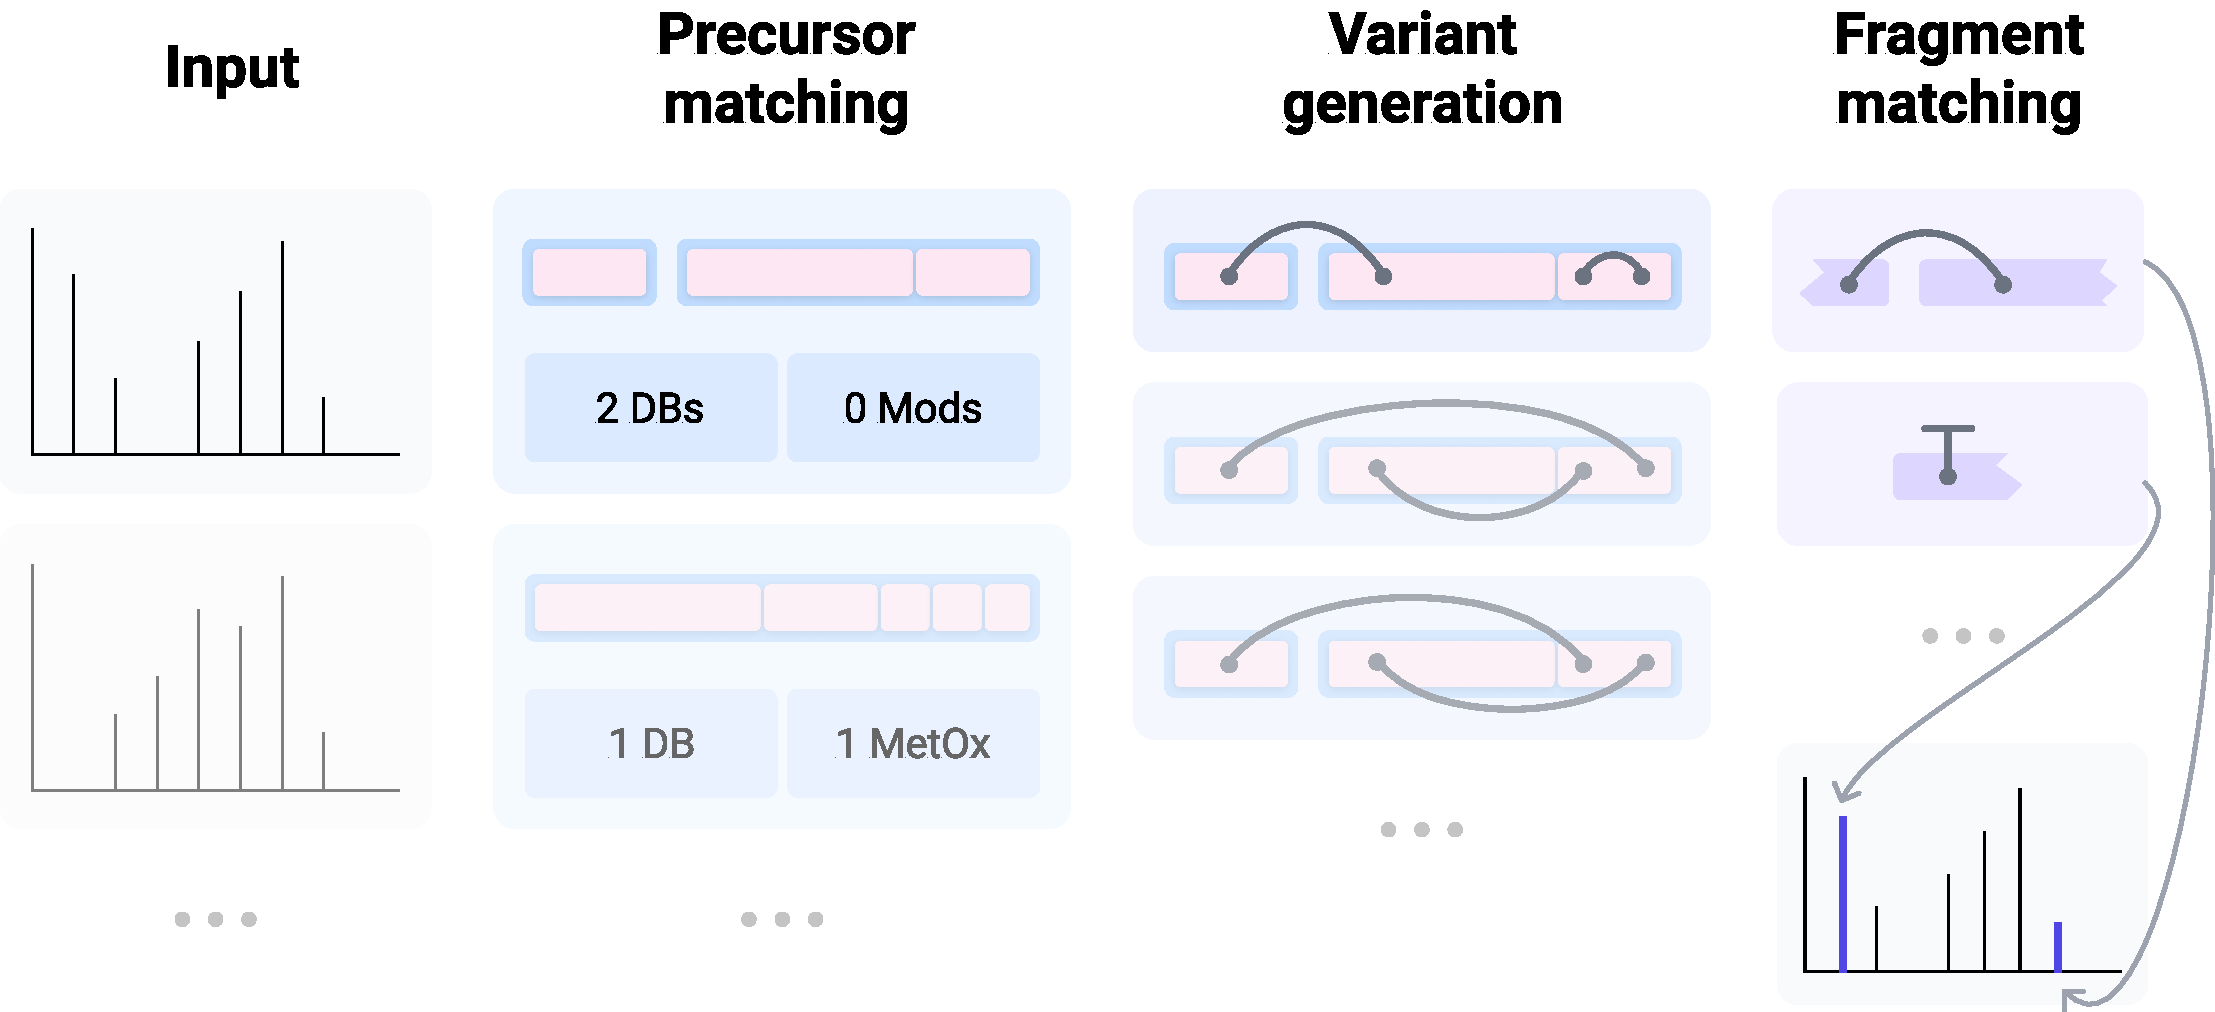
\includegraphics[width=\linewidth]{img/pipeline.pdf}
  \caption{The processing and assignment pipeline in Dibby, not including scoring and visualization. First, precursors are assigned to the provided spectra, then the precursors are used to generate \emph{variants}, and finally, fragments of the variants are assigned to the peaks in the spectra. Refer to the main text for definitions of each of the terms. Pink bits represent basal peptides resulting from protein digestion, or \emph{tryptides}, and the bigger blue rectangles around them represent \emph{segments}, longer peptides made of one or more \emph{tryptides}.}\label{fig:pipeline}

\end{figure}

\begin{figure}
  \centering
  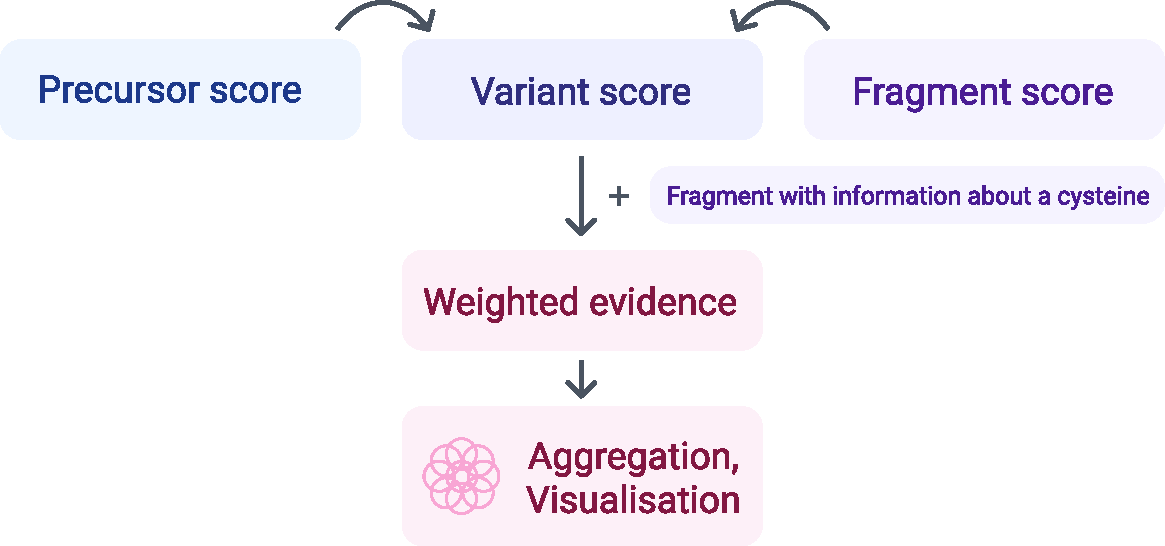
\includegraphics[width=0.75\linewidth]{img/score-calculation.pdf}
  \caption{This figure illustrates how the evidence about \gls*{db} linkage is weighted and aggregated. Our goal is to evaluate the evidence for each possible \gls*{db}; the evidence is gathered from the fragment assignments. To improve the quality of the evidence, Dibby tries to weed out false positive assignments by weighting evidence from each fragment by the score of its variant. The variant score is calculated from the precursor score and the score of assigned fragments belonging to the variant.}\label{fig:score-calculation}
\end{figure}


\subsection{Precursor assignment}

At the beginning, the protein undergoes a complete in-silico digestion, producing basal peptides that can not be digested any further; the protease of our choosing was trypsin, so we call these basal peptides \emph{tryptides}. As mentioned in the first chapter (\Cref{sec:trypsin}), a protease can sometimes miss a cleavage point, resulting in a peptide chain that is made from two (or more) contiguous basal tryptides. We call a chain of one or more tryptides a \emph{segment}. Due to the presence of \glspl*{db} in our samples, a \emph{precursor} is made out of one or more segments connected with inter-peptide \glspl*{db}\footnote{There can be additional \glspl*{db} connecting a segment to another segment, and there can also be intra-segment \glspl*{db}.}.


From the point of view of this stage of the algorithm, it matters not where the individual \glspl*{db} are located, because the different \emph{variants} are not distinguishable on the basis of precursor mass. Thus, for each precursor that it managed to assign to a spectrum, the output of the precursor matching algorithm only includes the following information:

\begin{itemize}
  \item The segments that are present in the precursor.
  \item The number of \glspl*{db} in the precursor.\footnote{The number of \glspl*{db} is always at least the number of segments minus 1.}, and, by extension, the number of alkylated cysteines in the precursor --- every cysteine that does not partake in a bond is considered alkylated. Notice the algorithm does not say anything about \emph{where} the bonds or alkylations are.
  \item The number of other amino acid modifications, for example methionine oxidations. The set of modifications that Dibby considers during precursor matching is configurable; these modifications are treated the same as ``variable'' modifications are treated in other software.
\end{itemize}


The precursor is built iteratively segment by segment, and the individual segments are built tryptide by tryptide, from left to right. First, given a target mass, the algorithm chooses a beginning of the first segment. After that the \textsc{FindPrec} function iteratively branches out to search the solution space for precursors with a theoretical mass within an error boundary around the target. A pointer to the list of tryptides is kept, and we will call the tryptide that is pointed to in some specific iteration of the function the ``current'' tryptide. As illustrated in \Cref{alg:findprec}, in each iteration, each of the following is attempted:

\begin{enumerate}
  \item Combine the \Var{Selected} segments with potential modifications and \glspl*{db} in such a way that together they have the correct mass. The valid combinations are found using the \textsc{Combine} function. \textsc{Combine} implements a divide and conquer algorithm for a modified subset sum problem, in which assignments that are within some error boundary of the target are also considered to be a valid solution.
  \item End the current segment (effectively simulating a protease cleavage just before the current tryptide) and begin a new one that begins on the current tryptide or later.
  \item Elongate the current segment by adding the current tryptide to it.
\end{enumerate}

The fact that the precursors (and their segments) are built strictly from left to right is a simple form of symmetry breaking --- that is, it prevents generating multiple equivalent symmetric solutions. Some further optimizations were added as well, mainly to prevent traversing a branch once we learn it can not provide any more solutions. Finally, the maximum number of segments can be specified, so that precursors containing too many segments are ignored, even though their mass would match the target.


\begin{algorithm}
  \begin{algorithmic}
    \Function{FindPrec}{$I, \mathit{Selected}, \mathit{Mass}, \mathit{Segments}, \mathit{Cys}, \mathit{Open}$}

    % \nb{There is no hanging disulphide bond from previous segments}
    \If{not $\mathit{Open}$}\label{alg:findprec:combinations} \Comment{No hanging \gls*{db} is present}
    \Upd{S}{\textsc{Combine} the segments with some mods to match \Var{TARGET}}
    \EndIf

    \If{$\mathit{Mass}$ is too high, or $i$ is at the end}
    \State return \Var{solutions} \Comment{There are no further solutions in this branch}
    \EndIf

    \If{not \Var{Open}, and $\mathit{Segments} > 0$, and $\mathit{Cys} > 0$}\label{alg:findprec:end}\Comment{Start a new segment}
    \For{every potential start of the next segment from $I + 1$ onward}
    \Upd{S}{\Call{FindPrec}{$\mathit{start}, \mathit{Mass} - \ce{H2}, \mathit{Segments} - 1, \mathit{Cys} - 1, \mathrm{True}$}}
    \EndFor
    \EndIf

    \nb{Elongate the current segment by one tryptide}
    \Decl{t}{the $I$-th tryptide}
    \Decl{open'}{False if this tryptide had any cysteines, otherwise same as \Var{Open}}

    \Upd{S}{\Call{FindPrec}{$I + 1, \mathit{Mass} + t_{mass}, \mathit{Segments}, \mathit{Cys} + t_{cys}, open'$}}\label{alg:findprec:elongate}

    \State return the list \Var{S}
    \EndFunction
  \end{algorithmic}
  \caption{A basic structure of the precursor matching algorithm with the respective branching points, implemented in pseudocode. Implementation details as well as some optimizations were omitted for brevity.}\label{alg:findprec}
\end{algorithm}

\subsection{Fragment assignment}

This part of the program assigns fragments to the peaks from the spectra. The fragments are generated in-silico from the precursors that were assigned by the algorithm from the previous section. There is an additional in-between processing step that generates all possible \emph{variants} that a matched precursor could represent. A \emph{variant} is a set of segments with precisely defined \glspl*{db}, while a precursor only provides information about the number of \glspl*{db}, not their positions. Similarly to how precursors are constructed from cross-linked segments, and the segments from basal tryptides, fragments can also be broken down to smaller pieces; we call these pieces \emph{cuts}. A \emph{cut} is a contiguous slice of one precursor segment.\footnote{The set of interconnected cuts that constitute the fragment forms a connected subgraph in the variant graph.} The fragment is build cut by cut, although this time the cuts are not added from left to right.

To explain the mode of operation of \textsc{FindFrag}, we have to introduce the notion of \emph{pivots}. The algorithm builds a cut residue by residue, until it encounters a cysteine connected by a \gls*{db} to another cysteine in the variant. When the algorithm makes the decision to keep the bond intact, the fragment will definitely have to contain the other cysteine, and possibly some other residues that neighbour it in its segment. The other cysteine is thus added to a list of \emph{pivots}, and when the current cut is ended, the algorithm jumps to a next pivot in the list and builds a new cut around it.

For an outline of the algorithm, see \Cref{alg:fragment}. At the start, a beginning for the first cut of the fragment is chosen from a list of valid beginnings in the variant. The \textsc{FindFrag} function then iteratively explores the solution space by branching out, similarly to \textsc{FindPrec}. The algorithm jumps back and forth between segments, following the directions of \glspl*{db} in the variant, building cuts around pivots. The algorithm stops when it runs out of pivots, runs out of residues in the variant, or when its mass becomes too high. As illustrated in \Cref{alg:fragment}, in each iteration, the algorithm attempts to do the following:

\begin{enumerate}
  \item Combine the masses of the \Var{Selected} cuts and some available variable modifications to obtain a fragment with a mass that is within the error boundary around the target mass. In case of a success, add this fragment (that is, this combination of cuts and modifications) to a list of solutions.
  \item If the current residue is a cysteine partaking in a \gls*{db} that we have not seen yet, branch out. In one branch, break the bond, adding asymmetric modifications to both of the cysteines, and keep the bond intact in the other branch, adding a new \emph{pivot} to the list of pivots.
  \item Elongate the current cut by adding the next residue to it. The ``next residue'' is simply the following residue in the segment in which the current cut is made. If there is no ``next residue'', end this cut, and jump to the next pivot. If there is no pivot to jump to, end this branch of the algorithm.
  \item End this cut prematurely (in the middle of a segment), that is, simulate a peptide bond dissociation in the precursor. Jump to the next pivot, if there is any, or end this branch of the algorithm.
\end{enumerate}

The algorithm keeps track of all residues that are part of the current fragment, in order not to add any residue twice. The maximum number of bond cleavages can be specified, so that fragments that result from more cleavages in the variant are ignored by the algorithm.

In addition to what is shown in the pseudocode, Dibby accounts for neutral losses, variable amino acid modifications, multiple numbers of bond cleavages, asymmetric \gls*{db} cleavages, and a range of potential fragment charges. Consequently, Dibby is in theory able to identify any protein fragment, including the kinds summarized in \Cref{fig:bond-types}.

\begin{algorithm}
  \begin{algorithmic}
    \Function{FindFrag}{$I, \mathit{BreaksLeft}, \mathit{Ends}, \mathit{Mass}, \mathit{Pivots}$}

    \Decl{solutions}{an empty list}

    \Decl{can end}{the end would not be premature, or \Var{BreaksLeft} $> 0$}
    \If{\Var{I} is in \Var{Ends}, and also \Var{can end}}

    \If{can \textsc{Combine} the cuts with some mods to match \Var{TARGET}}\label{alg:fragment:combine}
    \Decl{solutions}{the current \Var{solutions} with any of the new ones added}
    \EndIf

    \If{there is some pivot $\mathit{p}$ in $\mathit{Pivots}$}\label{alg:fragment:end}
    \Decl{startrange, endrange}{the valid cut range around \Var{p}}
    \Decl{pivots'}{\Var{pivots} with the pivot \Var{p} removed}
    \Decl{breaks'}{\Var{BreaksLeft}, possibly one less if the end is premature}
    \For{every valid cut start in \Var{startrange}}
    \Decl{S}{\Call{FindFrag}{$\mathit{start}, \mathit{breaks'}, \mathit{endrange}, \mathit{Mass}, \mathit{pivots}$}}
    \Decl{solutions}{the current \Var{solutions} concatenated to \Var{S}}
    \EndFor
    \EndIf

    \EndIf

    \If{the \Var{I}-th residue is a cys partaking in a \gls*{db} we have not seen yet}\label{alg:fragment:cysteine}

    \nb{Break the bond\ldots}
    \If{we have some breaks to spare}
    \State add the current cysteine to the broken bond counter, then\ldots
    \Decl{mass'}{the current \Var{Mass} added to the mass of the \Var{I}-th residue}
    \Decl{S}{\Call{FindFrag}{$I + 1, \mathit{BreaksLeft} - 1, \mathit{Ends}, \mathit{mass'}, \mathit{pivots}$}}
    \Decl{solutions}{the current \Var{solutions} concatenated to \Var{S}}
    \EndIf
    \nb{\ldots or keep it intact}
    \Decl{pivots'}{add the other end of the bond to \Var{Pivots}}
    \Decl{mass'}{the mass of the bond, $\ce{H2}$, subtracted from \Var{Mass}}
    \Decl{S}{\Call{FindFrag}{$I + 1, \mathit{BreaksLeft}, \mathit{Ends}, \mathit{mass'}, \mathit{pivots'}$}}

    \Decl{solutions}{the current \Var{solutions} concatenated to \Var{S}}

    \Else
    \nb{Continue elongating this cut}\label{alg:fragment:elongate}
    \Decl{mass'}{the current \Var{Mass} added to the mass of the \Var{I}-th residue}
    \Decl{S}{\Call{FindFrag}{$I + 1, \mathit{BreaksLeft}, \mathit{Ends}, \mathit{mass'}, \mathit{pivots}$}}
    \Decl{solutions}{the current \Var{solutions} concatenated to \Var{S}}
    \EndIf
    \State return the list \Var{solutions}
    \EndFunction
  \end{algorithmic}
  \caption{A pseudocode implementation of the basic functionality of the fragment matching algorithm.}\label{alg:fragment}
\end{algorithm}

\subsection{Precursor scoring and result visualization}\label{sec:scoring}

As illustrated in \Cref{fig:score-calculation}, a score of the precursor assignment is combined with scores from the fragment assignment to score the variants. Every fragment that contains a cysteine --- either alkylated or as a part of a \gls*{db} --- is treated as evidence for that specific state of that specific cysteine. The evidence from every fragment is weighted by the score of the variant from which the fragment was made, the results are aggregated and visualized. The scoring is vital for proper function of the program (see \Cref{fig:scoring-metric}); otherwise, the many false positives overwhelm the signal from true positives.

\paragraph{Precursor scoring} The score for a precursor \(P\) is computed as \[\textsc{PrecursorScore}(P) = \frac{1}{1 + \mathcal{w}_P \cdot (\mathrm{variants}_P, \mathrm{mc}_P, \mathrm{mass}_P, \mathrm{error}_P)^T},\] where \(\mathcal{w}_P\) is a vector of weights, \(\mathrm{variants}_P\) is the number of different variants that can be generated from \(P\), \(\mathrm{mc}_P\) is the maximum number of missed cleavages among its segments, \(\mathrm{mass}_P\) is its mass, and \(\mathrm{error}_P\) is the ppm error of the assignment. All of these attributes of are normalized before the score is computed. In this thesis we set \(\mathcal{w}_P = (32, 4, 4, 4)\).

\paragraph{Fragment scoring} The score for a fragment \(F\) is computed as \[\textsc{FragmentScore}(F) = \frac{1}{1 + \mathcal{w}_F \cdot (\mathrm{charge}_{F}, \mathrm{mods}_F, \mathrm{error}_F)^T},\] where \(\mathcal{w}:F\) is a vector of weights, \(\mathrm{charge}_F\) is the charge of the fragment, \(\mathrm{mods}_F\) is the total number of its mods (including neutral losses), and \(\mathrm{error}_F\) is the ppm error of the assignment. All of these attributes are normalized before the score is computed. In this thesis we set \(\mathcal{w}_F = (16, 4, 4)\).\footnote{Our values for \(\mathcal{w}_P\) and \(\mathcal{w}_F\) are aiming to reduce the exploitation of the flexibility of the matching system by large precursors and fragments.}

\paragraph{Variant scoring} The score of a variant \(V\) is computed as \begin{align*}
  \textsc{VariantScore}(V) & = \textsc{PrecursorScore}(\mathrm{precursor}_V)                                                        \\
                           & + w_f \cdot \operatorname{median} \set{ \textsc{FragmentScore}(F) \given F \in \mathrm{fragments}_V }.
\end{align*} In this thesis we use \(w_f = 1/2\).

\paragraph{Score aggregation} For every potential \gls*{db} \(B = (u, v)\) the following evidence score is computed  from the assigned fragments, \[\textsc{DBEvidence}(B) = \sum_{\substack{ \text{assigned} \\ \text{fragment } F }} \textsc{VariantScore}(\mathrm{variant}_F) \cdot [B \in \mathrm{bonds}_F], \] where \(\mathrm{bonds}\) is a set of \glspl*{db} that are present in the fragment. Similarly, for every cysteine \(C\) an alkylation score is computed, \[\textsc{AlkylationEvidence}(C) = \sum_{\substack{ \text{assigned} \\ \text{fragment } F }} \textsc{VariantScore}(\mathrm{variant}_F) \cdot [C \in \mathrm{alkcys}_F],\] where \(\mathrm{alkcys}\) is a set of alkylated cysteines that are present in the fragment.

\paragraph{Visualization} The aggregated evidence is plotted independently for each disulphide bond and --- in the case of alkylation --- for each cysteine (for an example, see \Cref{fig:lys}). The evidence for a bond \((u, v)\) is visualized separately in each direction, \(u \to v\) and \(v \to u\). The evidence for the edge \(u \to v\) is normalized in the context of every other bond \(u \to x\), and the evidence for alkylation of the cysteine \(u\). No further interpretation is done to keep the plots as close to the raw assignment data as possible. In addition to those two plots, plots of ground truth data are shown, representing the theoretical true state of the analysed protein. Alkylation evidence is illustrated by a border around the cysteine.

\subsubsection{Utilization of the AT and RAT results in differential analysis}\label{sec:diff}

Evidence plots are generated for the AT and RAT samples. Bonds that produce strong evidence in the RAT data, where in reality there should be no \glspl*{db} present, are deemed to be prone to generating false positives. For an example, see the bond \((75, 114)\) in the top-right-corner plot in \Cref{fig:lys}. We expect the same bond to generate a lot of false positive signal in the AT sample, too. Thus, we would like to penalize variants with this specific bond. This can be done by adding the \gls*{db} to a blacklist that gets checked by the precursor and fragment scoring functions. The effect of this basic differential analysis is illustrated in \Cref{fig:pdfa-lys-at-rat-diff}.

\subsubsection{Results interpretation}\label{sec:interpretation}

Due to the nature of the visualization, we say a bond \((x, y)\) has been \emph{identified} if and only if there is plenty of evidence for the \emph{bidirectional} connection between cysteines \(x\) and \(y\); in the plot, both of the arrows have to be green. For an example of an identified bond see \((72, 119)\) and the edges connecting those two cysteines in \Cref{fig:genova}.

If only one of the arrows is green, the existence of the bond is \emph{not} confirmed, because we have stronger evidence of the other cysteine being in a different configuration. For an example of this, see \(381 \to 119\) in the same figure. In this case, the evidence for the bond \((119, 381)\) is stronger than evidence for any other state of the cysteine \(381\), however, that is not the case for the cysteine \(119\). Namely, the cysteine \(119\) has another configuration with stronger evidence: the above-mentioned \gls*{db} \((72, 119)\). In cases such as this, further investigations into the data should be made, to determine whether this is caused by the algorithm, or due to a mistreatment of the data during measurement.
\chapter{Results and discussion}

In this chapter we present the results of \gls*{db} characterization in two measured proteins, and one in-silico generated dataset. We also provide some supporting data justifying our choice of scoring metric and the design of the matching algorithms. Finally, we evaluate the results, concluding that many \glspl*{db} are successfully identified, although there are many false positive fragment matches.

\section{Dibby scores reflect false positive fragment assignments}

In the proteins we analysed, the theoretical positions of \glspl*{db} are known. We call a fragment (and by extension, the whole variant) that contradicts the knowledge about \gls*{db} positions a \emph{bad} fragment. We have evaluated our variant scoring metric on four different datasets (\gls*{lys}, \gls*{lip}, \gls*{genova}, and \gls*{bsa}), separately on good and bad variants; the results are shown in \Cref{fig:scoring-metric}. A clear difference between the median variant score of the bad and the good variants can be seen.

\begin{figure}
  \centering
  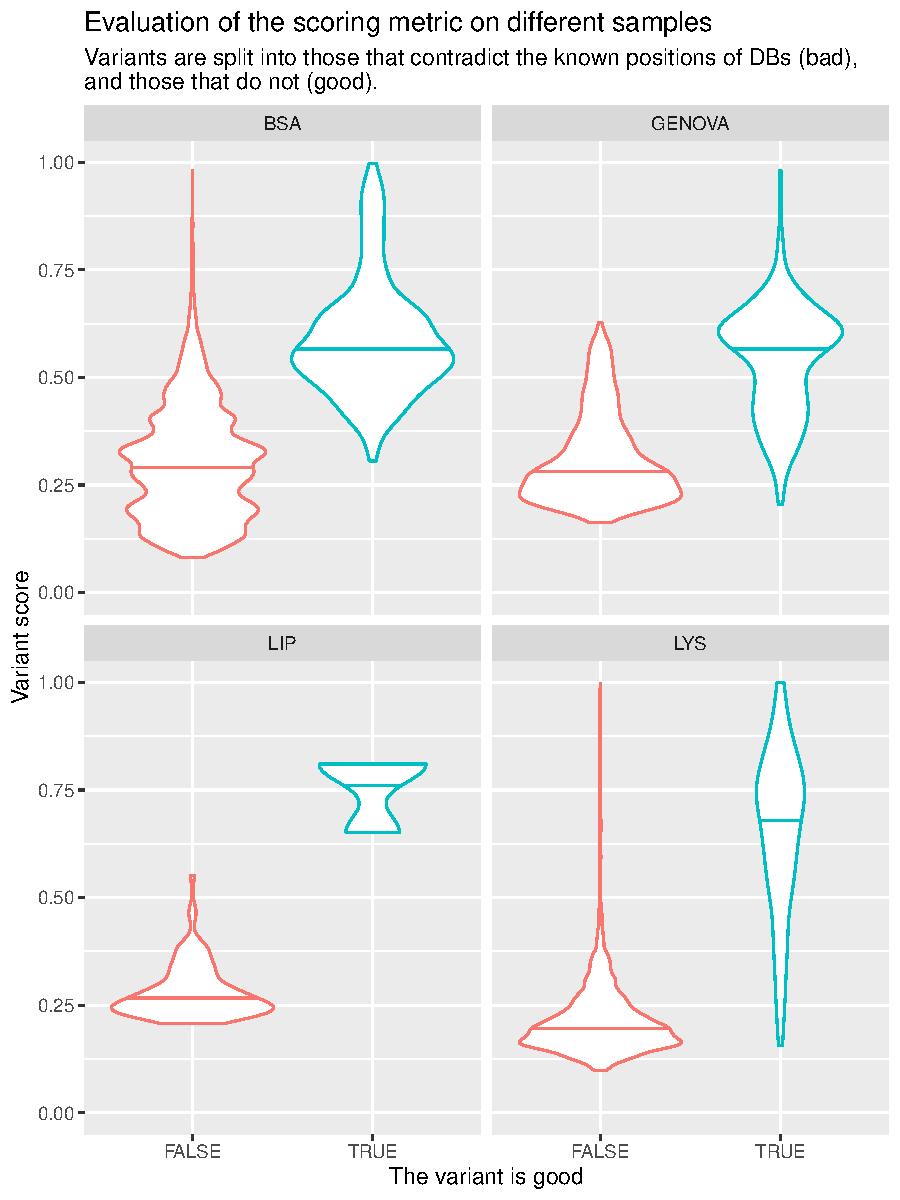
\includegraphics[width=0.85\linewidth]{img/scoring-metric-evaluation.pdf}
  \caption{Scoring metric evaluation on datasets from four different samples. Individual data points represent different assigned variants, that are grouped based on whether they contradict expert knowledge about \gls*{db} positions. The box plots illustrate that the separation is usually relatively good, but as we can see from the data points, there are still a lot of (in theory) non-existent variants with a high score. This can partly be attributed to \gls*{db} scrambling. The lack of data in the \gls*{lip} sample is discussed in the text. (\gls*{bsa} = bovine serum albumin, \gls*{lys} = lysozyme, \gls*{lip} = lipase, \gls*{genova} = an in-silico generated ovalbumin dataset)}\label{fig:scoring-metric}
\end{figure}

Additionally, we further reduce the influence of false positive matches on the results by blacklisting \glspl*{db} that are prone to generating false positive evidence. This process is described in detail in \Cref{sec:diff}. The effect of this differential analysis is illustrated on the example of the \gls*{lys} sample in  \Cref{fig:lys-at-rat-diff}.

\begin{figure}
  \centering
  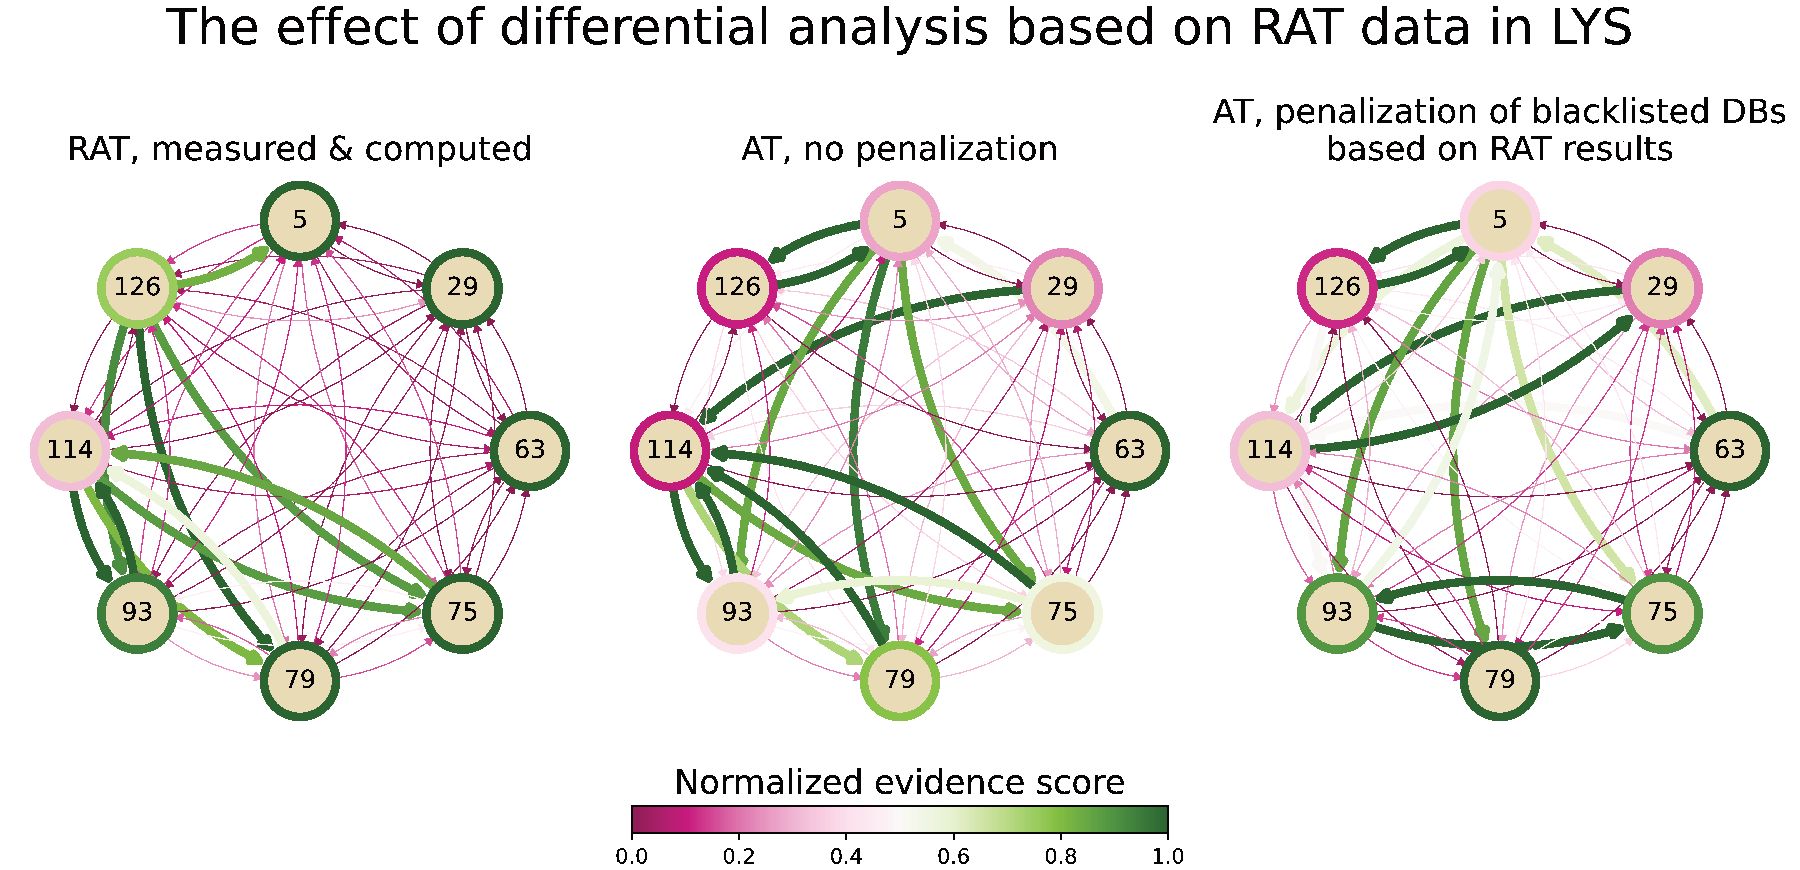
\includegraphics[width=1\linewidth]{img/pdfa-lys-at-rat-diff.pdf}
  \caption{On the left, the evidence for \gls*{db} positions in an RAT sample is visualized. Because the RAT sample should not contain any \glspl*{db}, we conclude that the edges with high evidence are false positives, and are likely to be carried-over to the analysis of the AT sample. The unmodified evidence from AT sample is depicted in the middle of the figure --- we can see that a lot of the edges from RAT are indeed visible here as well. Thus, we penalize the evidence coming from variants with bonds that are visible in the RAT sample, in an effort to quench the influence of these false positives. This results in a much better prediction of the \gls*{db} positions, as can be seen in the rightmost plot, where three of the four true \glspl*{db} are identified: \((5, 126)\), \((29, 114)\), and \((75, 93)\).}\label{fig:lys-at-rat-diff}
\end{figure}

\section{Dibby identifies existing disulphide bonds}

A complete \gls*{db} analysis has been performed on three proteins, namely \gls*{lys}, \gls*{lip}, and \gls*{genova}\@. The analysis was initially run with vanilla settings. If there had been a strong evidence for a particular \gls*{db} in the RAT data, it was deemed to be prone to generating false positive signals. Consequently, its weight has been adjusted to 0.1, or 0.8, depending on the strength of its RAT evidence, and the analysis was run again.

The results from the second run of the analysis can be seen on the following figures: \Cref{fig:lys} (\gls*{lys}), \Cref{fig:lip} (\gls*{lip}), and \Cref{fig:genova} (\gls*{genova}). The top row shows data from RAT samples, the bottom shows data from AT samples, the left column shows the theoretical positions of the cysteine alkylations and disulphide bonds, and the right column shows the aggregated evidence. Alkylation evidence is illustrated by a border around the cysteine.

As is apparent from the images, Dibby generates a lot of false positive signal. However, the scoring and weighting of the evidence helps immensely, and some \glspl*{db} are still clearly identifiable; three in the \gls*{lys} sample (of the four total \glspl*{db}), one in the \gls*{lip} sample (of the three total \glspl*{db}), and one in the \gls*{genova} sample (the only \gls*{db} that is present).


\paragraph{Lysozyme} Three of the four \glspl*{db} have been identified (\Cref{fig:lys}). The evidence for the last \gls*{db} has been seen in only 7 good fragments, compared for example to the 2,534 good fragments of the bond \((5, 126)\). We are not sure what caused this stark disparity, and the causes should be more deeply investigated in the future. The evidence for the bond \((75, 93)\) is not as strong as for the other two, relative to the evidence for alkylations of the respective cysteines. \((75, 93)\) is objectively hard to identify, because there is no tryptic cleavage point between the cysteines. The fact that Dibby has been able to identify this bond foreshadows the power of its general assignment algorithm.

\begin{figure}
  \centering
  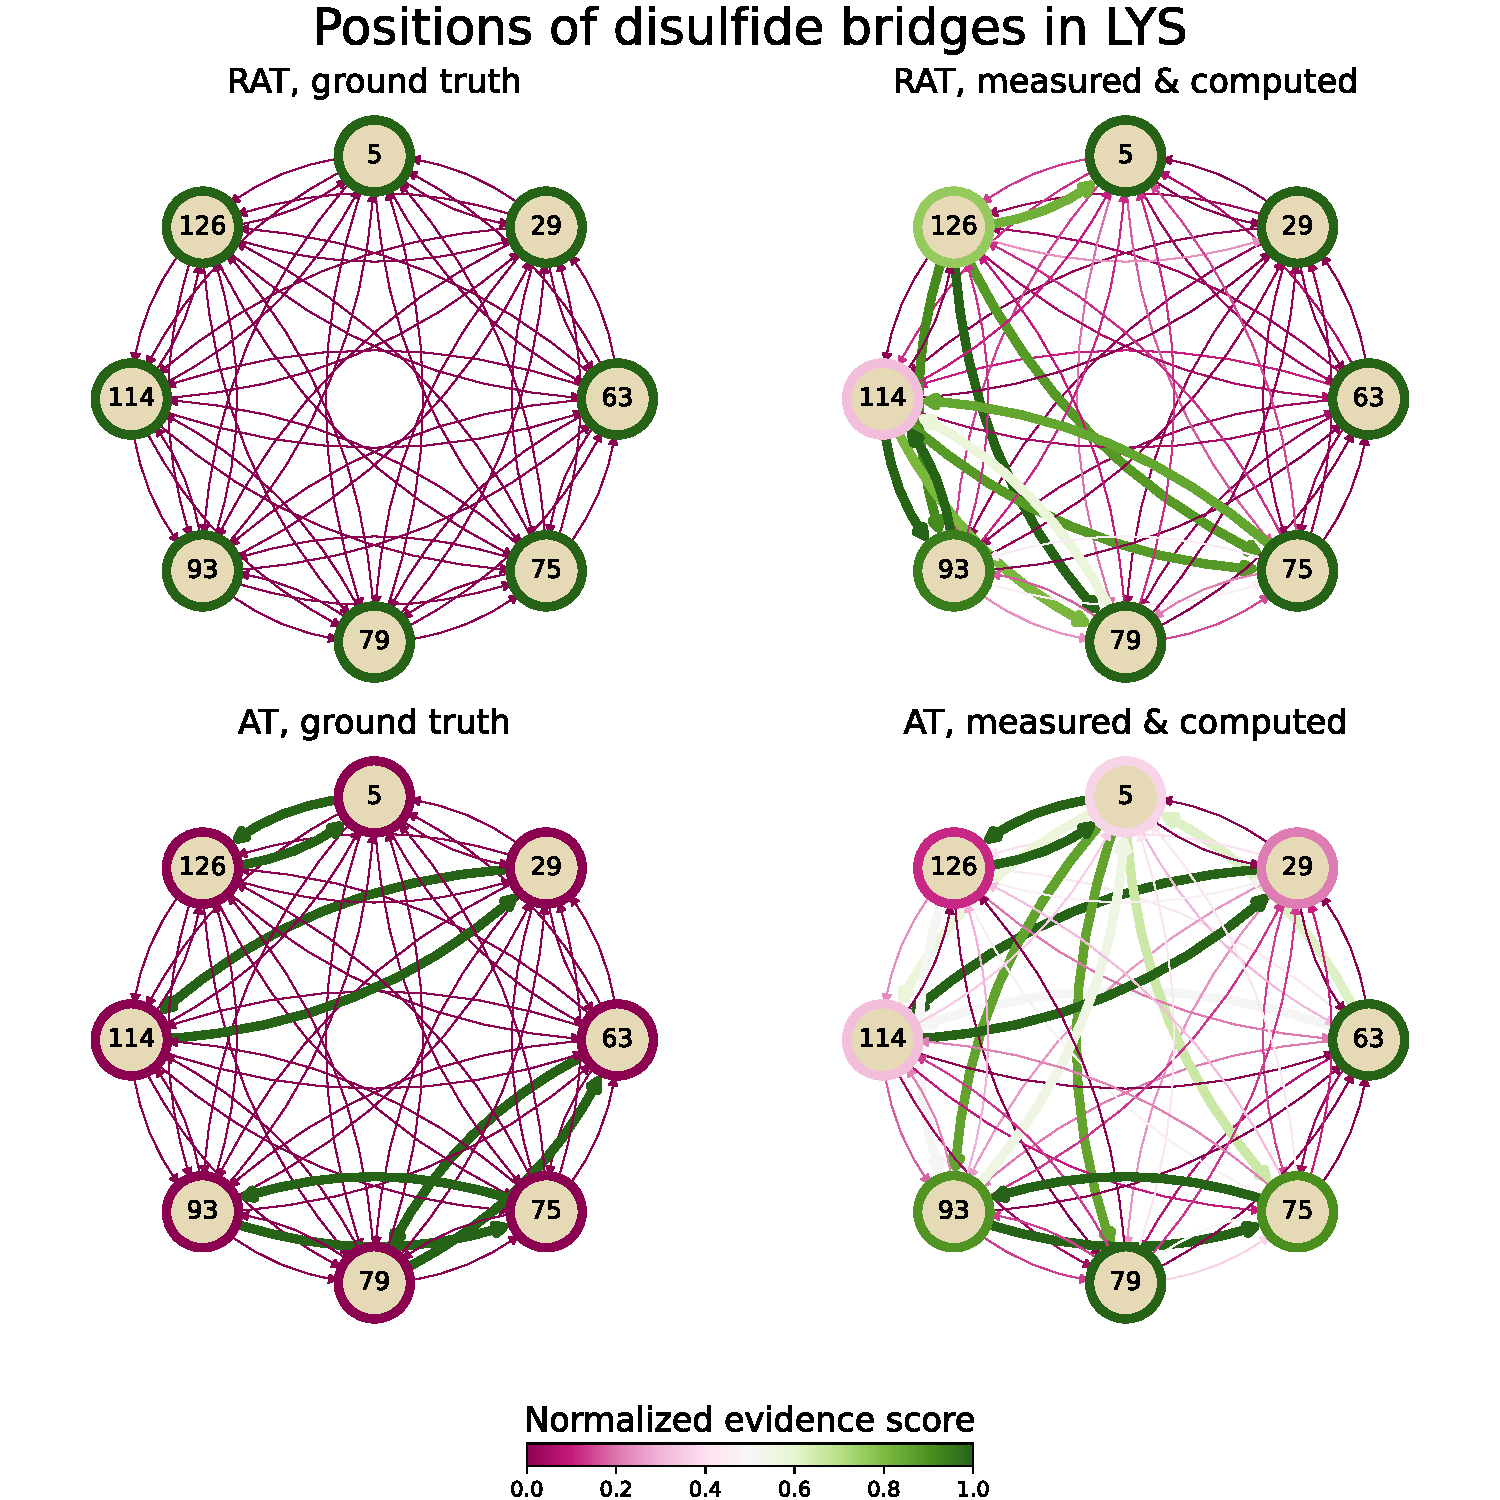
\includegraphics[width=0.9\linewidth]{img/pdfa-lys.pdf}
  \caption{The evidence for positions of \glspl*{db} and alkylations in lysozyme, weighted by variant score, and normalized. The bonds \((5, 126)\) and \((29, 114)\) are still clearly visible. The presence of the bond \((75, 93)\) is not so clear-cut; we also have strong signals about the cysteines being alkylated. This warrants further investigation. Finally, the evidence for bond \((63, 79)\) is practically not present, and both cysteines were deemed as alkylated. There are several one-directional false positives, however, we can safely ignore them (see \Cref{sec:interpretation} for details).}\label{fig:lys}
\end{figure}

\paragraph{Generated ovalbumin} Similarly to the lysozyme plots, some false positives had cropped up (\Cref{fig:lip}), though they did not manage to drown out the true evidence. The only present \gls*{db}, \((72, 119)\), has been successfully identified. There are some directed edges coming into the cysteine 119, however; the algorithm and the scoring system should be fine-tuned so that similar false positives do not slip through the cracks, or at least do not provide such a strong signal.

\begin{figure}
  \centering
  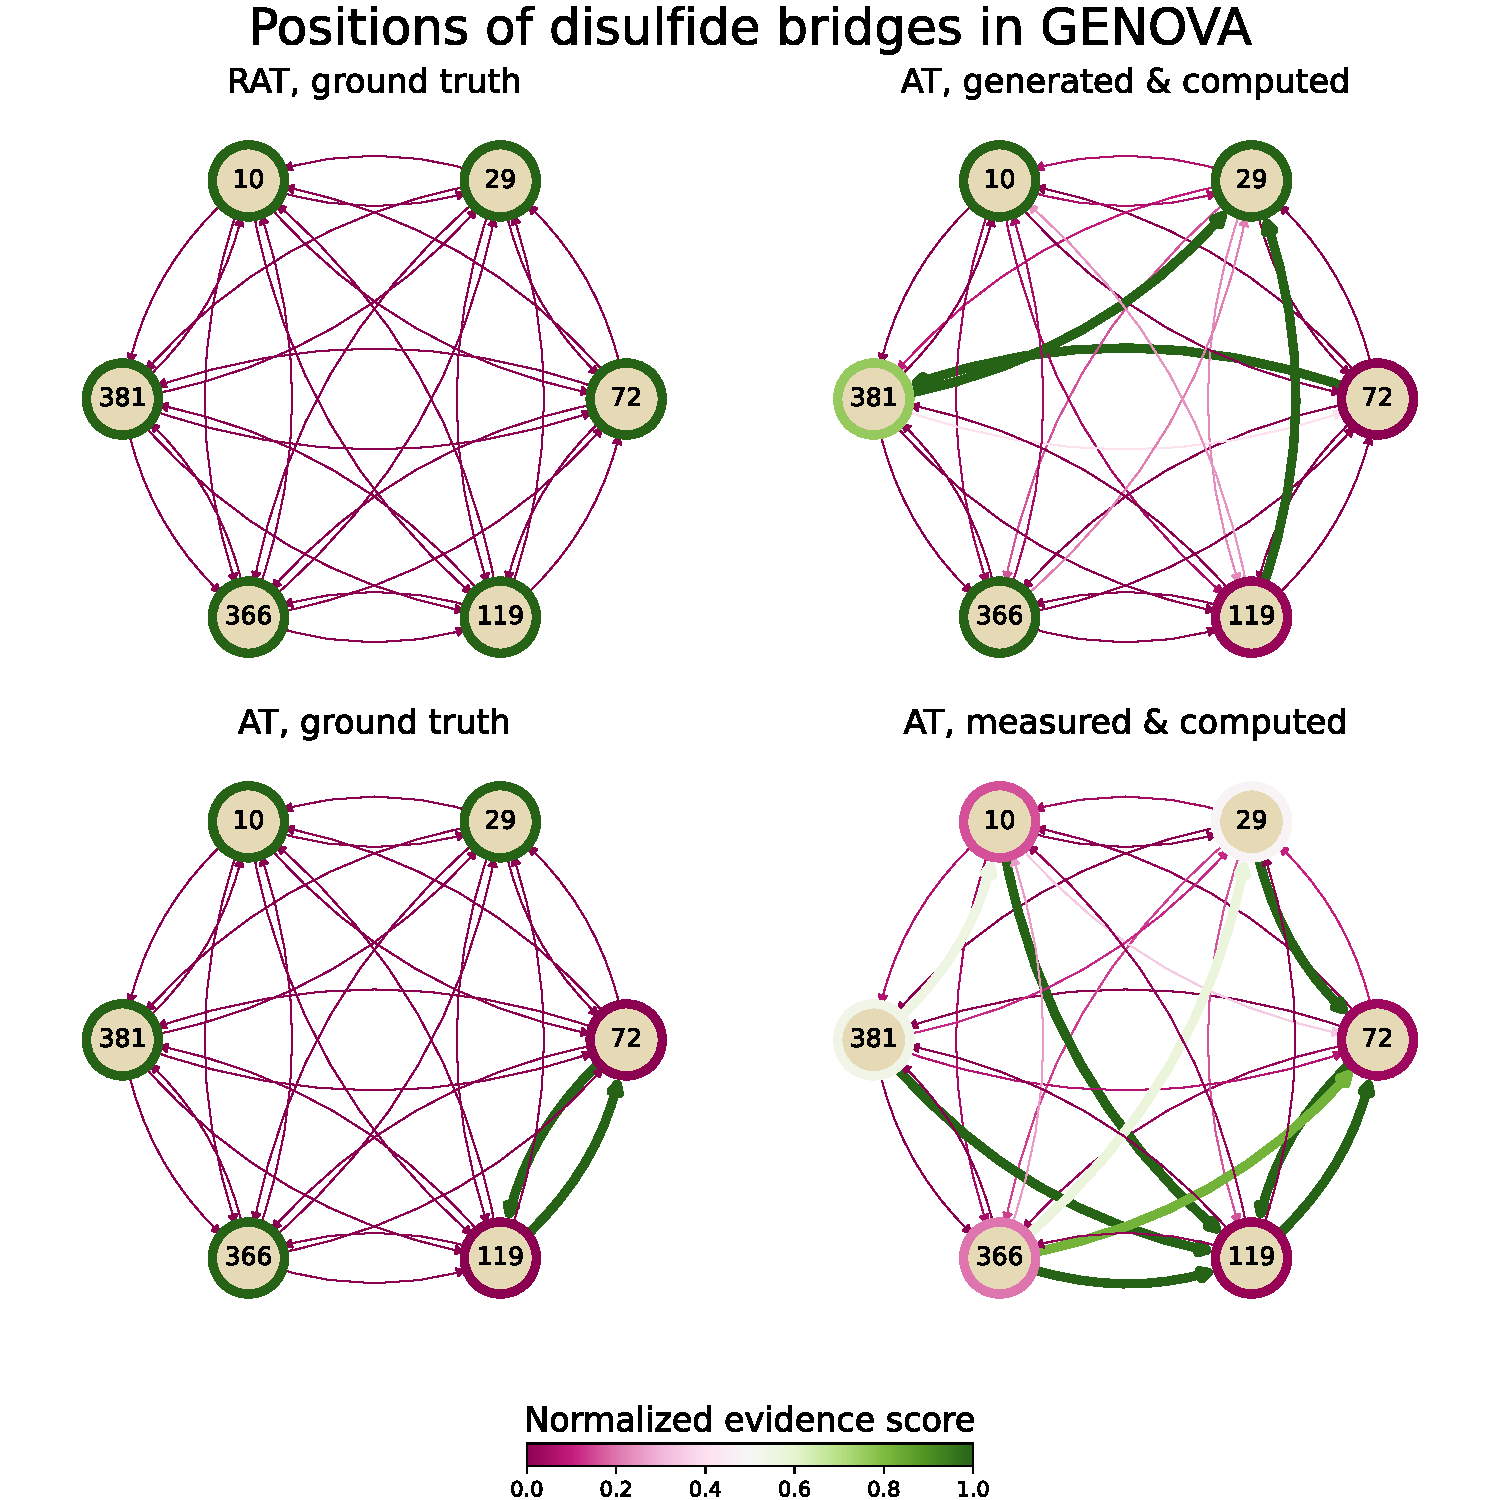
\includegraphics[width=0.9\linewidth]{img/pdfa-genova.pdf}
  \caption{The evidence for positions of \glspl*{db} and alkylations in in-silico generated ovalbumin, weighted by variant score, and normalized. Although there are some false positives, the only confirmed bidirectional bond is also the correct one: \((72, 119)\). There are several one-directional false positives, however, we can safely ignore them (see \Cref{sec:interpretation} for details).}\label{fig:genova}
\end{figure}

\paragraph{Lipase} Only one of the three \glspl*{db} has been identified in the \gls*{lip} sample (\Cref{fig:lip}). Interestingly, we have identified exactly zero variants containing the cysteines 271 and 295, alkylated or otherwise. To test whether this had been caused by a problem in the data or the algorithm, we have run a MSGF+~\cite{kim2014ms} analysis on the \gls*{lip} samples (and later on the other samples as well); the comparison with results from Dibby is in \Cref{tbl:measurements}. We can see that even MSGF+, a state of the art proteomic database search tool, had problems with \gls*{lip} data, suggesting an unidentified issue may have occurred during the sample preparation, rendering most of the \gls*{lip} data unusable.

\begin{table}[hb]
  \sffamily
  \begin{tabular}{@{}llllll@{}}
    \toprule
    \multicolumn{1}{c}{\multirow{2}{*}[-0.25em]{Sample}} & \multirow{2}{*}[-0.25em]{Scans} & \multicolumn{1}{c}{\multirow{2}{*}[-0.2em]{\begin{tabular}[c]{@{}c@{}}MSGF+\\Matches\end{tabular}}} & \multicolumn{3}{c}{Dibby matches}                       \\ \cmidrule(l){4-6}
    \multicolumn{1}{c}{}                                 &                                 & \multicolumn{1}{c}{}                                                   & Simple                            & Total & \glspl*{db} \\ \midrule
    \gls*{lys} AT                                        & 12479                           & 411                                                                    & 463                               & 2240  & 3/4         \\
    \gls*{lys} RAT                                       & 14517                           & 1216                                                                   & 2157                              & 2972  &             \\
    \gls*{lip} AT                                        & 13579                           & 21                                                                     & 12                                & 67    & 1/3         \\
    \gls*{lip} RAT                                       & 14177                           & 76                                                                     & 66                                & 131   &             \\
    \gls*{genova} AT                                     & 1606                            &                                                                        & 855                               & 3257  & 1/1         \\
    \gls*{genova} RAT                                    & 735                             &                                                                        & 770                               & 805   &             \\
    \gls*{bsa} AT                                        & 13856                           & 1495                                                                   & 1717                              & 48222 &             \\
    \gls*{bsa} RAT                                       & 14242                           & 1723                                                                   & 2684                              & 22133 &             \\ \bottomrule
  \end{tabular}
  \caption{Comparison of Dibby with MSGF+, a state-of-the-art database search tool for proteomics. MSGF+ can only identify peptides that are not cross-linked, or ``simple'' peptides; for this reason, we list the number of Dibby's simple assignments in addition to the total number of its assignments. Generally, Dibby identifies a bit more simple precursors than MSGF+, most of which are probably false positives. On the other hand, there are close to 0 false negatives. MSGF+ identified 16 times more precursors in the \gls*{lys} RAT sample than in \gls*{lip} RAT sample, and a similar effect is visible in the AT samples as well, suggesting there might be a problem in the \gls*{lip} data. The last column specifies how many \glspl*{db} Dibby identified, and what is the total number of \glspl*{db} in the protein.}\label{tbl:measurements}
\end{table}

\begin{figure}
  \centering
  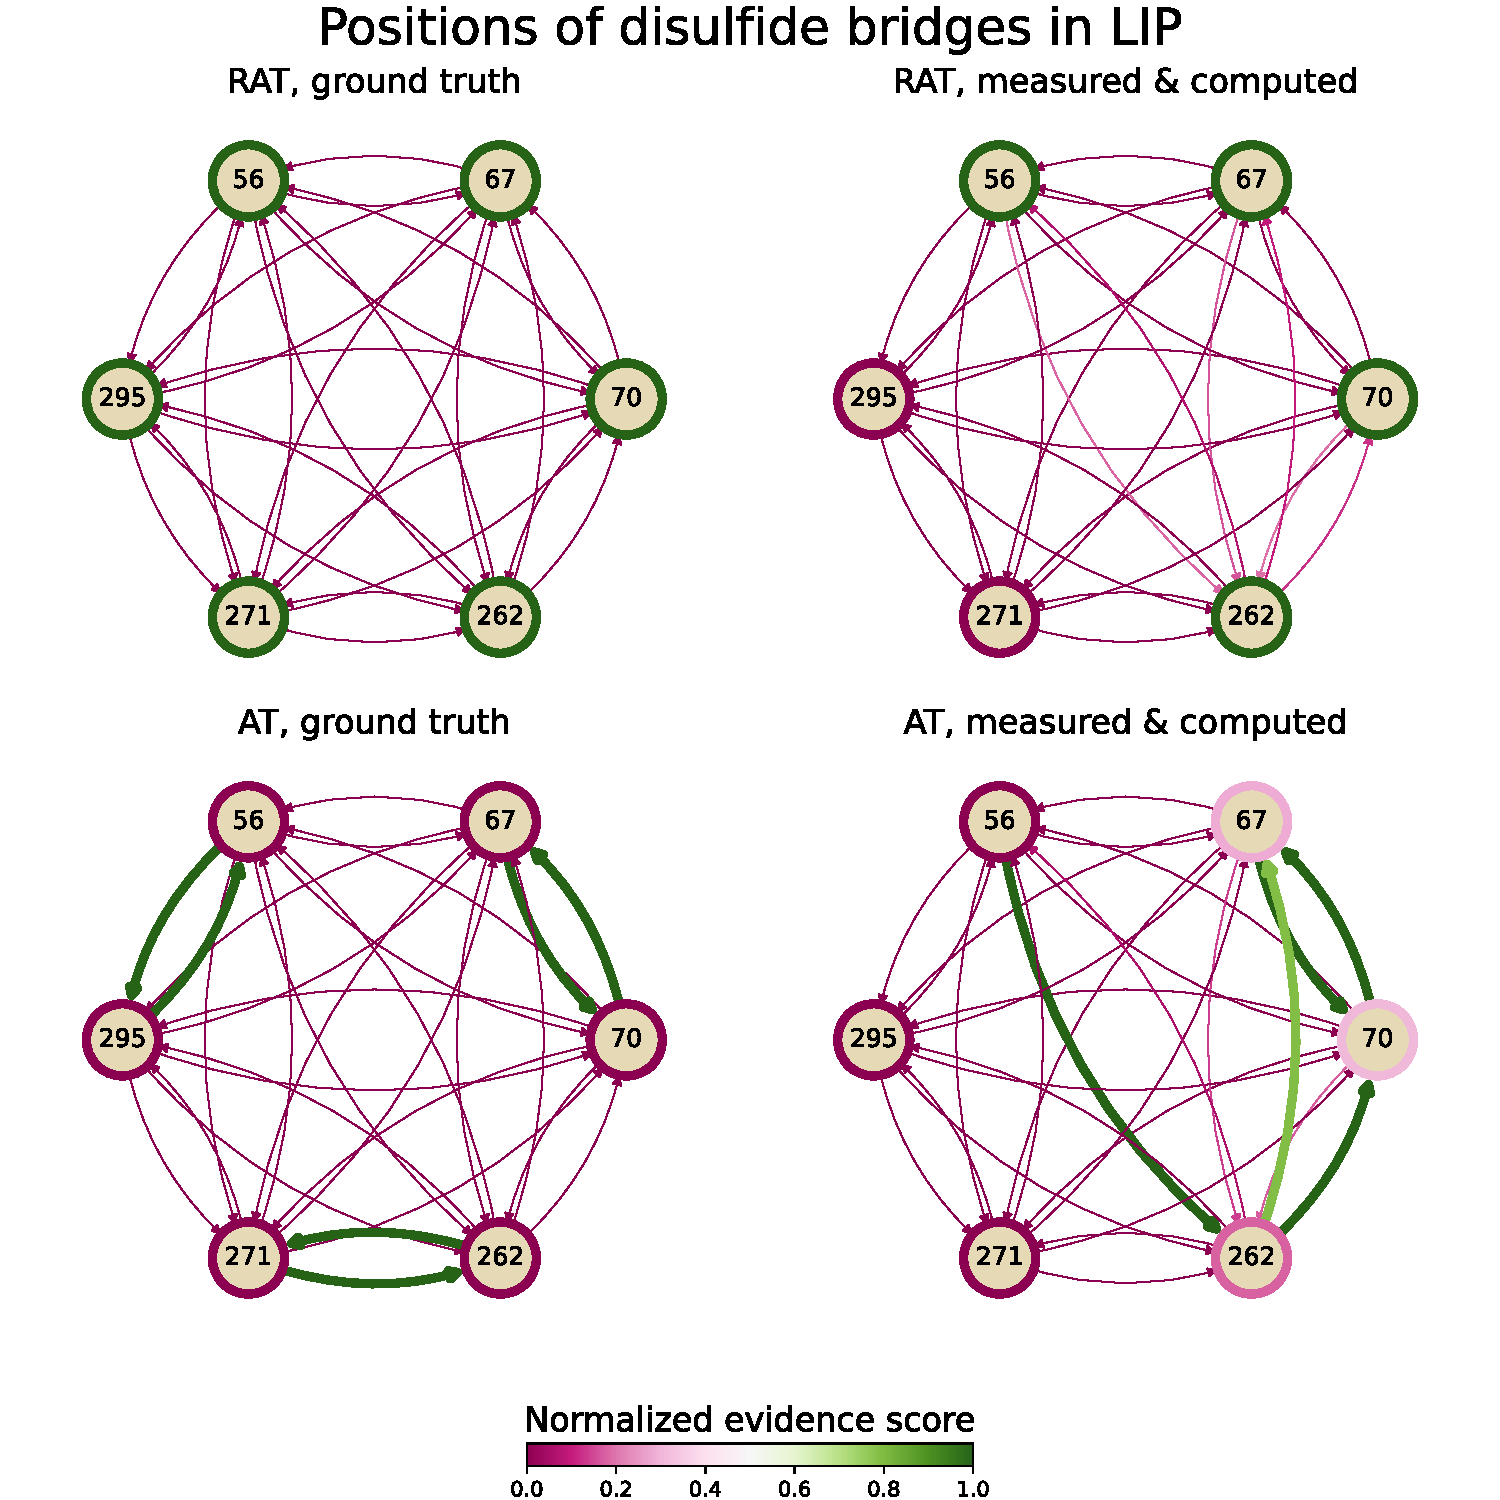
\includegraphics[width=0.9\linewidth]{img/pdfa-lip.pdf}
  \caption{The evidence for positions of \glspl*{db} and alkylations in lipase, weighted by variant score, and normalized. No fragments containing cysteines 271 and 295 have been assigned (neither in alkylated form, nor as a part of any disulphide bond); this leads us to believe that a part of the data has been lost, or otherwise damaged. Nonetheless, the bond \((67, 70)\) is successfully identified. There are several one-directional false positives, however, we can safely ignore them (see \Cref{sec:interpretation} for details).}\label{fig:lip}
\end{figure}

To conclude, the scoring metric separates good variants from the bad ones rather well. With the help of the scoring system, Dibby managed to sift through the large number of false positive fragment assignments, and successfully identified most of the true \glspl*{db} in the \gls*{lys} and \gls*{genova} samples. One true \gls*{db} has even been identified in \gls*{lip}, despite the problems in the \gls*{lip} dataset.


\section{Discussion}

In the discussion below, we do not consider the results obtained from the \gls*{lip} samples, because we could not interpret the data, due to an unidentified problem in the measurements.

\paragraph{Scoring} In order for the scoring metric to be useful, bad fragments and variants should generally have a lower score than good ones, presuming the measured data correlates with the expert knowledge about \gls*{db} positions. We have indeed found that the metric satisfactorily separates the good variants from the bad ones (see \Cref{fig:scoring-metric}), nonetheless there are still many bad variants with a high score, especially in the \gls*{bsa} and \gls*{lys} datasets. A possible explanation is that although \glspl*{db} that contradict expert knowledge should not be present in the data \emph{in theory}, due to \gls*{db} scrambling they \emph{are} present; subsequently, variants containing these bonds receive a high score because they match the measured data well, but are labelled as bad during our evaluation of the scoring metric (\Cref{fig:scoring-metric}). This hypothesis is further supported by the absence of the high-scoring bad variants from the generated \gls*{genova} dataset, in which no \gls*{db} scrambling has occurred.

\paragraph{\gls*{db} characterization} Despite the strong signal from false positive matches, and the complications resulting from \gls*{db} scrambling, most of the \glspl*{db} present in \gls*{lys} (\Cref{fig:lys}) and \gls*{genova} (\Cref{fig:genova}) have been identified. Especially important is the \gls*{lys} \gls*{db} \((75, 93)\), an intra-peptide \gls*{db} that would be hard to identify with other methods. This demonstrates the flexibility and raw matching power of the algorithm. However, more work needs to be done to lower the false discovery rate. After improvements in this area, and potentially some changes to the data preparation protocol, Dibby could be used to assist researchers with \gls*{db} mapping in proteins.

\paragraph{Manual analysis} In addition to the visualizations, a CSV file with the fragment assignments is generated by Dibby. This enables researchers to perform detailed manual analysis based on data from Dibby's matching algorithms, or to manually check the evidence for a specific \gls*{db} to verify the results. In the future, the match data could be used to perform automatic labelling of matched fragments, including complex internal fragments with multiple modifications and disulphide bonds, a task that is as of now still not solvable by any tool.

In conclusion, Dibby has managed to identify most \glspl*{db} from the analysed dataset, including one intra-peptide bond. We have also shown the importance of protease choice during the sample preparation phase by identifying variants that possibly resulted from \gls*{db} scrambling during tryptic digestion. Some of Dibby's shortcomings were highlighted, suggesting a topic for future research.

\chapwithtoc{Conclusion}

In this thesis we have reviewed the current approaches to disulfide bond mapping, and the different tradeoffs stemming from various choices regarding instrumentation, data preparation, and experiment design. We presented our own attempt at automatic computational disulfide bond characterisation, a program aiming to identify even complicated clusters of disulfide bonds, and intrapeptide disulfide bonds.

During the evaluation of the algorithm on real-world data we have inadvertently confirmed the occurence of DB scrambling during tryptic protein digestion. Furthermore, due to the high number of false positives among the assigned fragments, and the rather unsophisticated method of visualisation, a fair amount of manual labour is still needed to interpret the results. Another consequence of this is that the scoring metric needs to be quite complicated and opaque in order to weed out the false positve matches. Further research is needed to simplify the scoring metric --- a part of the solution will probably be a better utilisation of the data from RAT samples.

Despite these limitations, and the challenging conditions regarding the data we used, we have successfully demostrated the power of the program by identifying DBs in lysosyme, including one intra-peptide DB, and in our in-silico generated control dataset. We conclude that we have reached our goal of devising a general algorithm that is able to identify complicated crosslinked peptide fragments, but we consider it to be only a proof-of-concept at this stage of the development. Nonetheless, we think the approach of extensive matching of complicated peptide framgens could prove to be useful in mapping DBs in the future.

\section*{Future work}

It would be interesting to see how well the algorithm fares with data that are not digested with trypsin, to confirm whether the high number of unexpected identifications were due to the issue of DB scrambling during tryptic digestion. On this front, many other proteases would be viable, for example pepsin, or thermotrypsin~\cite{sung2016evaluation}. After a change in the sample preparation protocol, we expect the number of high-scoring ``bad'' variants to decrease, resulting in a stronger signal for the correctly identified DBs, and in a reduced number of false positives. The same outcome could also be achieved by optimising the scoring metric, and by more resourceful utilisation of the data from RAT samples. Last but not least, data from other fragmentation sources could be used to make the dataset richer.

Further work could be done to optimise Dibbi's performance. Divide and conquer algorithms lend themselves nicely to dynamic programming approaches, but the multitudes of information that the algorithm has to keep track of in our specific case --- such as neutral losses, amino acid modifications, cysteine alkylations, bond cleavages, error boundaries --- made it complicated to employ them. Nonetheless, should the program be deployed in real-life scenarios in the future, reductions in compute time would be needed. Additional speed-ups could be achieved by implementing the program in Julia\footnote{\url{https://julialang.org}} instead of Python.

Finally, due to its nature, Dibbi has very high sensitivity; so high in fact that it is almost detrimental due to the quantity of false positives, were it not for the elaborate scoring and weighting post-processing steps. However, Dibbi could be used to automatically label and analyse the various types of complex ions that show up in the fragmentation spectra, such as internal ions comprising of multiple crosslinked peptides. If the sample were prepared very carefuly, and the positions of DBs in the protein were known, this knowledge could be used to manually discard most of the false positives. In this way, Dibbi could be used to research and quantify the dissociation pathways of crosslinked peptides, potentially leading to more informed approaches to DB mapping in the future.

\ifEN
  \chapwithtoc{Bibliography}
\else
  \chapwithtoc{Seznam použité literatury}
\fi
\printbibliography[heading=none]


% \appendix
% \chapter{Using CoolThesisSoftware}

% Use this appendix to tell the readers (specifically the reviewer) how to use your software. A very reduced example follows; expand as necessary. Description of the program usage (e.g., how to process some example data) should be included as well.

% To compile and run the software, you need dependencies XXX and YYY and a C compiler. On Debian-based Linux systems (such as Ubuntu), you may install these dependencies with APT:
% \begin{Verbatim}
% apt-get install \
%   libsuperdependency-dev \
%   libanotherdependency-dev \
%   build-essential
% \end{Verbatim}

% To unpack and compile the software, proceed as follows:
% \begin{Verbatim}
% unzip coolsoft.zip
% cd coolsoft
% ./configure
% make
% \end{Verbatim}

% The program can be used as a C++ library, the simplest use is demonstrated in \cref{lst:ex}. A demonstration program that processes demonstration data is available in directory \verb|demo/|, you can run the program on a demonstration dataset as follows:
% \begin{Verbatim}
% cd demo/
% ./bin/cool_process_data data/demo1
% \end{Verbatim}

% After the program starts, control the data avenger with standard \verb-WSAD- controls.

% \begin{listing}
% \begin{lstlisting}
% #include <CoolSoft.h>
% #include <iostream>

% int main() {
% 	int i;
% 	if(i = cool::ProcessAllData()) // returns 0 on error
% 		std::cout << i << std::endl;
% 	else
% 		std::cerr << "error!" << std::endl;
% 	return 0;
% }
% \end{lstlisting}
% \caption{Example program.}
% \label{lst:ex}
% \end{listing}


% if your attachments are complicated, describe them in a separate appendix
%\include{attachments}

\openright
\end{document}
